\documentclass[12pt,a4paper]{article}
\usepackage[utf8]{inputenc}
\usepackage{amsmath}
\usepackage{amsfonts}
\usepackage{amssymb}
\usepackage{mdframed}
\usepackage[english]{babel}
\usepackage{wrapfig}
\usepackage{verbatim}
\usepackage{graphicx}
\usepackage{pdfpages}
\usepackage[titletoc]{appendix}
\usepackage{longtable}
\author{Bergar Simonsen}
\title{Jolie cloud computing}
\setlength{\parindent}{0cm}
\usepackage{listings}
\usepackage{color}

\definecolor{dkgreen}{rgb}{0,0.6,0}
\definecolor{gray}{rgb}{0.5,0.5,0.5}
\definecolor{mauve}{rgb}{0.58,0,0.82}

\lstset{frame=tb,
  language=Java,
  aboveskip=3mm,
  belowskip=3mm,
  showstringspaces=false,
  columns=flexible,
  basicstyle={\small\ttfamily},
  numbers=left,
  numberstyle=\tiny\color{gray},
  keywordstyle=\color{blue},
  commentstyle=\color{dkgreen},
  stringstyle=\color{mauve},
  breaklines=true,
  breakatwhitespace=true
  tabsize=3
}

\begin{document}
\pagestyle{empty}
\begin{abstract}
For cloud computing to be successful in the future, PaaS frameworks for deploying cloud services are essential since service developers need a platform on which they can deploy their services.\\
Existing PaaS cloud frameworks do not support automatic handling of non-functional aspects, such as authentication. In most cases they are limited to a single platform and only allow the deployment of software written in a fine number of programming languages.\\
By building on the existing JSOA framework, it is possible to create a PaaS framework with automatic authentication handling, which runs on all major platforms and supports deployment of services written in all or most popular programming languages. In addition to allowing developers to extend the framework to support additional programming languages and platforms.\\
This thesis presents the extended JSOA framework. By taking advantage of its heterogeneity, scaling the framework to support multiple programming languages, while still allowing for further scaling, is achieved. The JSOA framework runs natively on the Windows and Linux platforms and automatically handles authentication independently of the deployed services.

\end{abstract}
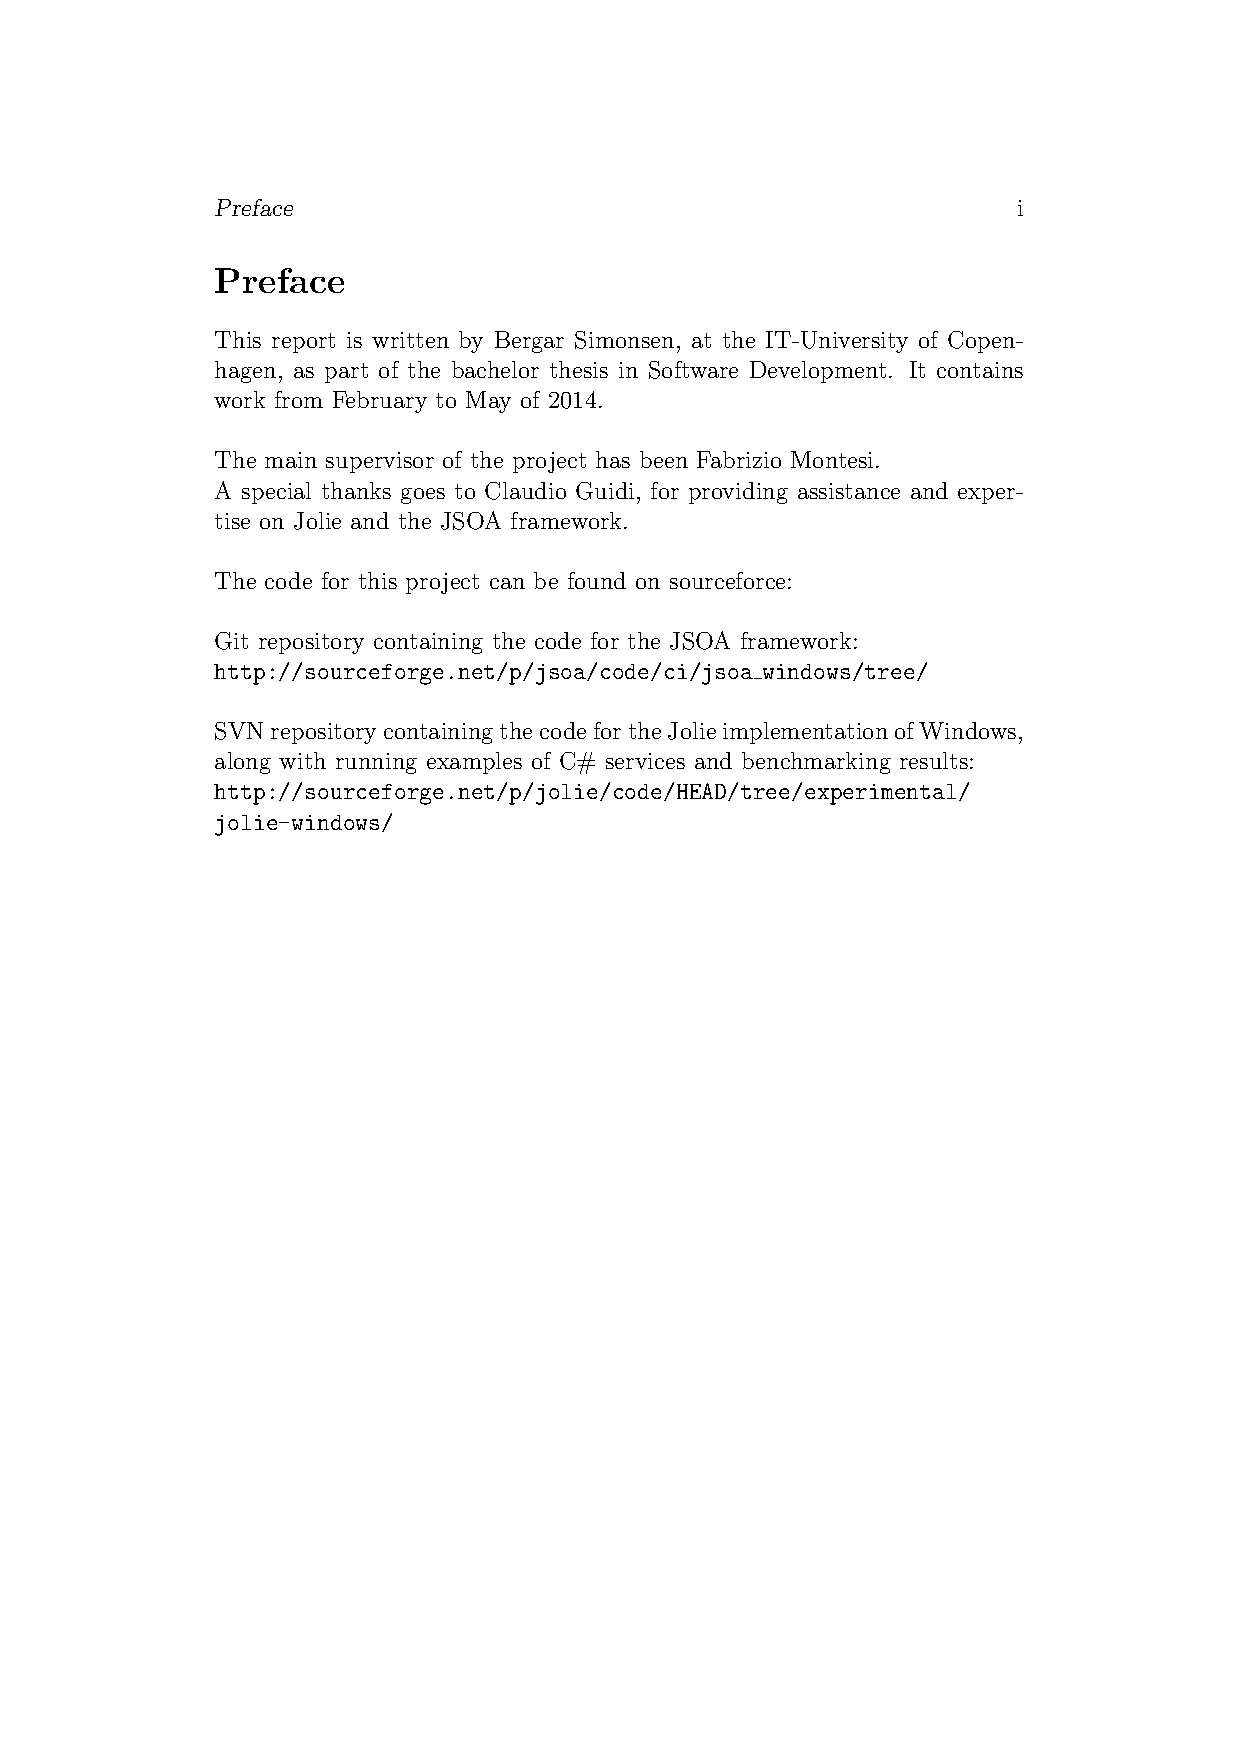
\includepdf[pages={1}]{introduction/introduction.pdf}
\tableofcontents

\pagestyle{plain}
\pagenumbering{arabic}
\newpage
\section{Introduction}\label{sec:Introduction}
In recent years, cloud computing has become a hot topic in modern computer science. The ability to host a service in a single cloud somewhere on the internet is very appealing, and is a subject that is under constant research and development.\\
Cloud computing consists of multiple servers that are connected to each other via the internet. Combining all these servers, allows developers to deploy software which then can be accessed from anywhere in the world. These servers supply the processing power needed to perform certain tasks, freeing the clients from doing the heavy computing work which might needed for a service. \\

Cloud computing can be divided into three layers. Infrastructure as a service (IaaS), Platform as a service (PaaS) and Software as a service (SaaS)\footnote{see \texttt{section \ref{subsec:CloudComputing}} for more details on cloud computing}. \\
IaaS deals with the hardware infrastructure, such as the underlying server or virtual machine, network infrastructure and so on. PaaS is the computing layer. Operating system, programming environments, databases are all running on the PaaS layer. The final layer, SaaS, is the actual service running on the cloud framework. This could be anything from email server applications, games, and other software. 

\subsection{Structure of the thesis}\label{subsec:StructureOfTheReport}
This thesis is structured as follows:
\begin{itemize}
\item Section \ref{sec:Introduction} gives an introduction to the thesis, followed by a problem description, aim of the thesis, thesis statement and finally the contributions of the project

\item Section \ref{sec:Background} provides some background information on cloud computing and the Jolie programming language

\item Section \ref{sec:Methodology} is the methodology used in the thesis. Technical analysis and implementation, followed by a running example and evaluation of the JSOA framework are analysed in this section

\item Section \ref{sec:Conclusion} reports the conclusions and future work for the project
\end{itemize}

\subsection{Problem description}\label{subsec:ProblemDescription}
For cloud computing to be successful in the future, PaaS frameworks are essential since developers need frameworks on which they can deploy their software. \\
Currently there are a number of PaaS frameworks on the market. Microsoft Azure\cite{azure_website}, Amazon EC2\cite{ec2_website} and Google App Engine\cite{google_app_engine_website} are some notable examples. Although these examples are widely used, they do have some limitations. \\
The first limitation is that developers are tied to having their entire cloud at a single provider, e.g., these frameworks do not allow having the IaaS at one place, and have a PaaS framework from another provider running on top. Another limitation is support for multiple programming languages and platforms. Although these examples mentioned here do support multiple platforms and a range of programming language, they do not allow developers to extend the framework, e.g., developers can not add additional programming languages or additional features to the framework.\\
In addition to the limitations mentioned above, most of the time these frameworks give the developer a platform for deploying software and nothing else. Everything, including non-functional tasks such as authentication, need to be implemented for each service. Some PaaS frameworks (e.g., Google App Engine) do offer APIs for authentication which aid developers with the implementation, but they still need to be handled by each service.\\

To the best of my knowledge, there is no PaaS framework which runs on all major platforms (e.g., Windows, Linux and OSX) and supports all major programming languages\footnote{This thesis defines popular programming languages as the major programming languages used today, e.g., Java, C\#, Objective-C, C etc.}, or at least have the ability to extend the framework to support a particular programming language. Neither is there a framework that supports those features mentioned here while also allowing the developer to abstract from non-functional tasks such as authentication.\\

\begin{mdframed}
\textbf{Problem statement} \\
Existing PaaS cloud frameworks do not support automatic handling of non-functional aspects, such as authentication. Neither do they support deployment and monitoring of services written in all major programming languages, or at least have the ability to be extended, by the developer, to support additional programming languages.
\end{mdframed}

\newpage
\subsection{Aim}\label{subsec:Aim}
The goal of this thesis is to contribute to a PaaS framework which runs on all major platforms and supports the deployment and management of software written in different programming languages. Particularly the more popular programming languages are important in order to give the framework a commercial appeal.\\
The framework needs to be heterogeneous in the sense that the framework can be distributed across multiple servers, and thus allowing scaling of the framework to support additional programming languages. \\
In addition to supporting multiple programming languages and platforms, the framework should handle most of the non-functional and administrative tasks so that developers of software services can abstract away from these features. These tasks include monitoring services as well as authentication. \\

\begin{mdframed}
\textbf{Aim}\\
To contribute to a general purpose PaaS framework which supports automatic handling of non-functional aspects such as authentication and integrate it with commercial programming languages to give a commercial appeal to the framework, while still allowing further extension to support additional languages and platforms.
\end{mdframed}

~\\
The methodology of this thesis will be to extend the existing JSOA\cite{jsoa_website} framework in order to create a PaaS framework which reaches the aim of the thesis.\\

There are a number of reasons why JSOA is a good starting point for developing such cloud frameworks: 

\begin{itemize}
\item \textbf{Solid foundation.} The JSOA framework is built for running on the Linux platform. Since JSOA is written in Jolie, which is built on Java, the foundation is already in place to make it platform independent.

\item \textbf{Working prototype.} JSOA is a working prototype which currently supports deployment of services written in Jolie, Java and Javascript. JSOA also currently has a working administration module so there is no need to implement this from scratch.

\item \textbf{Heterogeneous.} JSOA supports heterogeneous computing in the way that a single JSOA central control panel supports multiple "domains", each running on the same server or even distributed across multiple servers. This makes JSOA a good starting point for extending its functionality, while at the same time distributing it among multiple servers (see \texttt{section \ref{subsec:JSOA}}).

\item \textbf{Separate deployment from behaviour.} As stated, JSOA is built on Jolie. The very nature of Jolie makes it very easy to separate deployment from behaviour (see \texttt{section \ref{subsec:Jolie}}). Because of this, Jolie does not differentiate between local communication, and communication with services running on remote servers. This makes Jolie, and by extension JSOA, ideal for developing distributed systems. 
\end{itemize}

As stated above, the foundation of JSOA is already in place and therefore makes it an ideal starting point for this thesis.

\subsection{Thesis statement}\label{subsec:ThesisStatement}
This thesis attempts to find a solution to the issue regarding cross-platform, multilingual PaaS cloud frameworks and to help service developers by automatically handling some non-functional aspects. \\

\begin{mdframed}
\textbf{Thesis statement}\\
By extending the JSOA framework and make it platform independent, and by taking advantage of it's heterogeneity, one can develop a PaaS framework which runs on all major platforms, supports the running of services written in all major programming languages and allow service developers to abstract away from non-functional aspects such as authentication.
\end{mdframed}

~\\
More specifically, this thesis attempts to port the JSOA framework to the Windows platform, making it runnable on both Linux and Windows, and add the C\# language to its list of supported programming languages.\\
In addition, an attempt to integrate authentication into the framework, freeing service developers from having to handle authentication in every service, is made.

\newpage
\subsection{Contributions}\label{subsec:Contributions}
This thesis provides three main contributions. \\

\textbf{Windows and C\# integration}\\
JSOA currently supports deployment of services written in Jolie, Java and JavaScript and runs on the Linux platform.\\
The first contribution is to integrate JSOA to the Windows platform. Although JSOA is built on Jolie which is platform independent, it is designed for running on Linux, and therefore there has not been any effort put into making it platform independent, so some changes need to be made to JSOA in order for it to run natively on Windows. \\
The first contribution is to integrate JSOA to run on the Windows platform, and support the deployment of services written in the .NET (C\#) programming language.\\

\textbf{Authentication}\\
Currently, JSOA does not offer any authentication. All authentication for deployed services need to be implemented ad-hoc.\\
The second contribution will be to add authentication to the JSOA framework, allowing service developers to abstract away from handling any authentication on each service. \\

\textbf{Evaluation}\\
The third contribution is to develop a proof-of-concept service, written in C\#. This proof-of-concept service will be used to evaluate the JSOA framework and demonstrate that the above contributions are met.

\newpage
\section{Background}\label{sec:Background}
\subsection{Cloud computing}\label{subsec:CloudComputing}
As stated in the introduction, a cloud system basically is collection of servers or virtual machines, connected by the internet, that form a "cloud" which services can be deployed on. This definition is very rough, so this section will give a more thorough definition of what cloud computing actually is. \\

The National Institute of Standards and Technology (NIST) defines cloud computing as:
\begin{quote}
\emph{Cloud computing is a model for enabling convenient, on-demand network access to a shared 
pool of configurable computing resources (e.g., networks, servers, storage, applications, and 
services) that can be rapidly provisioned and released with minimal management effort or 
service provider interaction. This cloud model promotes availability and is composed of five 
essential characteristics, three service models, and four deployment models.}\cite{nist}
\end{quote}

As stated by the NIST, cloud computing consists of \emph{"five 
essential characteristics, three service models, and four deployment models."}\cite{nist} The following section will describe these characteristics, service models and deployment models. \\

\textbf{Characteristics}\\
In order to be qualified as a cloud system, there are some characteristics which need to be fulfilled in the system.
\begin{itemize}
\item \textbf{\emph{Always on}} \\
The first of these characteristics is that the service is always running. What this means in practice is that a user can, at any time, connect to the service in order to use storage, processing power, or other resource without requiring any human interaction.

\item \textbf{\emph{Broad network access}} \\
The capabilities (or resources) of the service are available through the internet at any time. In addition, they are available through any standard device that has access to the internet (e.g PCs, mobile phones and PDAs)

\item \textbf{\emph{Resource sharing}} \\
Another core characteristic of cloud computing is resource sharing.\\
The cloud is organized in such a way that multiple clouds or services running in the cloud share a large resource pool. This resource pool is then assigned to which ever service requires it. For example if a service is attracting more users at a certain time, additional resources from the resource pool are assigned to the service. When the demand falls back to normal, the resources are put back in the pool.

\item \textbf{\emph{Elasticity}} \\
Elasticity means that a service can expand or shrink at any time.\\
When a service is deployed in the cloud, the deployer does not have to allocate a specific amount of storage or bandwidth to the service but these can be expanded at any time.

\item \textbf{\emph{Monitoring}} \\
Cloud systems monitor their running service in order to determine how many resources are required. Monitoring is essential for \emph{Resource sharing} and \emph{Elasticity} to work properly without human interaction.
\end{itemize}

\textbf{Service models}\\
As also stated in the introduction, cloud computing can be divided into three layers, or service models:
\begin{itemize}
\item \textbf{\emph{Infrastructure as a service (IaaS)}} \\
IaaS' supply consumers with computing power. This includes processing power, storage, network and other computing resources. The consumer can then deploy and run software on this service. An example of software running on IaaS is the operating system.

\item \textbf{\emph{Platform as a Service (PaaS)}} \\
The primary task of the PaaS is to provide the deployment environment to the consumer. Deployment environment include a framework for running software, programming languages and compilers, databases, and other related software.\\
The PaaS abstract away from the underlying infrastructure, but often has some control of the service deployed on top of the PaaS. Monitoring of running services is an example.

\item \textbf{\emph{Software as a Service (SaaS)}} \\
SaaS is the actual cloud service deployed on the cloud framework. This service could be anything from an email application to social networks.\\
These services are available for users to interact with, through their clients (PC and mobile phone), via the internet.
\end{itemize}

\textbf{Deployment models}\\
Deploy models define how a cloud is deployed and to what extent users have access to the cloud system.
\begin{itemize}
\item \textbf{\emph{Public cloud}} \\
This is the most common deployment model. Public clouds are available for all users who have access to the internet.

\item \textbf{\emph{Community cloud}} \\
The community cloud is a cloud that is owned by several organizations or companies. An example of this could be a large company, that consists of several smaller companies, where all share a cloud for internal storage and communication.

\item \textbf{\emph{Private cloud}} \\
The private cloud belongs to a single organization or company. The private cloud is inaccessible for anyone except the owner. This deployment model is often used when the owner deals with sensitive data, but needs to share the data internally.

\item \textbf{\emph{Hybrid cloud}} \\
Hybrid clouds are a combination of the other three deployment models. For example, if a large company which owns a lot of smaller companies, needs allow the smaller companies to see data, but not be able to edit it, a hybrid cloud is ideal. The cloud would be a community cloud in the sense that multiple companies share the same cloud, while being a private cloud at the same time since only the head company can edit the data.
\end{itemize}

\newpage
\subsection{Jolie}\label{subsec:Jolie}
Jolie is a service-oriented programming language built on Java. \\
What makes Jolie an ideal choice for programming distributed systems, is its ability to separate deployment from behaviour. \\
This section will describe some of the important Jolie features which will be used in this thesis. For more information about Jolie, see \cite{jolie_website}. \\

A standard Jolie service is divided into two parts, the deployment, which deals with how the service is deployed and how it communicates with other services. The second part, the behaviour, deals with what the service does, e.g., the actual work performed by the service.

\begin{lstlisting}[caption={Separation of deployment and behahaviour in Jolie},label={lst:jolieDeploymentBehaviour}]
inputPort inputPort_1 {
	Location: "socket://localhost:9999"
	Protocol: sodep
	Interfaces: interface_1 }
main { /* some code */ }
\end{lstlisting}

\texttt{Listing \ref{lst:jolieDeploymentBehaviour}} shows an example Jolie service. Lines 1 - 4 show an input port, which is the deployment part, while line 5 shows the main operation, which is the behaviour part. \\
In the example above, the input port can be considered to be like a \texttt{socket listener} \cite{java_socket_listener} in Java. This analogy is not 100\% correct since Jolie input ports support multiple technologies (e.g., bluetooth, local memory etc.). What they all do have in common is that the input port listens for incoming connections at the specified location. \\
This particular input port listens for request on localhost, port 9999 and uses the Sodep\cite{jolie_protocols} protocol (lines 2-3), and implements the interface interface\_1 (line 4). A Jolie output port has the same syntax as the input port, only the \emph{inputPort} keyword is changed to \emph{outputPort}. \\
The second part, line 5, is the behaviour of the service. This contains the actual work the service performs. \\
\texttt{Listing \ref{lst:jolieDeploymentBehaviour}} demonstrates one of the major strengths of Jolie. Not only does it elegantly separate the deployment from the behaviour, but it also completely abstracts from which technology is used. Whether it communicates with a file in the same folder, a remote server or a bluetooth device, it makes no difference to the input port, or the rest of the service.\\ 

\textbf{Data types} \\
Data types in Jolie are designed as an XML like tree structure. \\
\begin{lstlisting}[caption={Jolie data types},label={lst:jolieDataTypes}]
type DataType: void {
	.id: int
	.value: int
	.domain: void
		.address: string
		.port: int }
		
dataType.id = 1;
dataType.value = "some value";
dataType.domain.address = "localhost";
dataType.domain.port = "8000"

<DataType>
	<id> 1 </id>
	<value> some value </value>
	<domain>
		<address> localhost </address>
		<port> 8000 </port>
	</domain>
</DataType>
\end{lstlisting}

\texttt{Listing \ref{lst:jolieDataTypes}} shows a Jolie data type and the same data type implemented in XML. This structure allows Jolie to easily implement complex, tree like data structures. \\
Lines 1 - 6 show how the data type is structure. Lines 8 - 11 show how the data type is used in practice. Finally, lines 13 - 20 show how the same data type would be implemented in XML.\\

In Jolie, every data type is a dynamic array. In practice, this means that there is no syntactical difference between a "regular" data type, and a list. Note that line 8 in \texttt{Listing \ref{lst:jolieDataTypes}} implicitly is referring to the first element in the dynamic array, e.g., datatype.id = 1 is the same as datatype.id[0] = 1.\\
The only difference between a list and a single object in Jolie, is in the type definition.

\begin{lstlisting}[caption={Jolie dynamic array},label={lst:jolieDynamicArray}]
type Person: void { .name: string, .phoneNumber*: string }
\end{lstlisting}

\texttt{Listing \ref{lst:jolieDynamicArray}} shows the syntactical difference between a single value and a dynamic array. The Person type has a name (string) and any number of phoneNumbers, specified by the * notation.\\

\textbf{Embedding} \\
Jolie supports embedding of other services. This means that when developing a Jolie service, the developer can embed another service inside that service, which allows the running of a service as a sub-service, creating a hierarchy of services. Embedding currently supports services written in Jolie, Java and JavaScript. \\
\texttt{Listing \ref{lst:jolieEmbedding}} shows how embedding in Jolie is used. Line 1 shows the syntax, while line 2 shows a specific example of how embedding is used.

\begin{lstlisting}[caption={Jolie embedding},label={lst:jolieEmbedding}]
embedded { Language : path [ in OutputPort ] }
embedded { Jolie: "service_1.ol" in outputPort_1 }
\end{lstlisting}

\textbf{Aggregation} \\
Aggregation in Jolie allows the creation of proxy services that can forward invocations to other services. Aggregation is purely related to deployment and has nothing to do with the behaviour of the service. Aggregation allows  an input port to aggregate an output port, creating a bridge between them. 
\begin{lstlisting}[caption={Jolie aggregation},label={lst:jolieAggregation}]
outputPort outputPort_1 {
	Location: "socket://localhost:8991"
	Protocol: sodep
	Interfaces: Interface_1 }
 
inputPort inputPort_1 {
	Location: "socket://localhost:8009"
	Protocol: http
	Aggregates: outputPort_1 }
\end{lstlisting}
\texttt{Listing \ref{lst:jolieAggregation}} shows an example of aggregation. When a request is sent to \texttt{inputPort\_1} via the http protocol, the request is forwarded to the aggregated \texttt{outputPort\_1} via the sodep protocol. \\
Using aggregation makes it easy to develop large, distributed systems. For example, \texttt{inputPort\_1} from the example above could aggregate multiple output ports, allowing the input port to forward requests to multiple different location with just a single line of code. \\

\newpage
The following example (\texttt{Listing \ref{lst:aggregationAndEmbeddingExample}}) demonstrates how embedding and aggregation works in Jolie. 
\begin{lstlisting}[caption={Aggregation and embedding example},label={lst:aggregationAndEmbeddingExample}]
// Service A
outputPort B { 
	Location: "serviceB.location"
	Protocol: http Interfaces: Interface_B }
outputPort C {
	Location: "serviceC.location"
	Protocol: soap Interfaces: Interface_C }
outputPort D { Interfaces: Interface_D }
embedded { Jolie: "serviceD.ol" in D }
inputPort A { 
	Location: "socket://sample.location:99"
	Protocol: sodep Aggregates: B, C, D }
\end{lstlisting}
Assume that we have four services A, B, C and D. Services B, C, D are independent services and service A is described above (\texttt{Listing \ref{lst:aggregationAndEmbeddingExample}}) \\
As seen in \texttt{Listing \ref{lst:aggregationAndEmbeddingExample}}, service A has three output ports, one for each service, and a single input port. Output port C and B are "regular" output ports, while output port D \emph{embeds} a service (service D). Input port A aggregates all three output ports. 

\begin{figure}[h!]
  \centering
    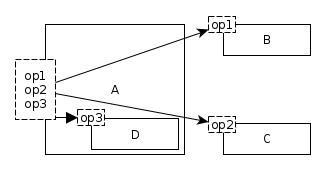
\includegraphics[width=0.5\textwidth]{../figures/jolie_aggregation_and_embedding_example.png}
  \caption{Aggregation and embedding}
  \label{fig:aggregationAndEmbedding}
\end{figure}

\texttt{Figure \ref{fig:aggregationAndEmbedding}} shows how the communication flow is. A client sends a request to service A with three operations. Op1 is forwarded to service B, op2 forwarded to service C and op3 forwarded to service D via their respective output ports (\texttt{Listing \ref{lst:aggregationAndEmbeddingExample}}). \\
Notice that the aggregator service completely abstracts away from the fact that output port D embeds an independent service. Aggregators only deal with output ports and do not care how the service is structured. \\
Using aggregators allows Jolie to build large, distributed systems with very low coupling between modules. \\

\textbf{Courier} \\
Courier sessions allow the composition of services independently from the context they belong to. Courier session can add extra procedures (for example authentication) to any service, without having any effect on the service itself.\\
Couriers rely on aggregation and allow the aggregator to handle a special session for the incoming request. Couriers allow services to overload operations, and add extended data to the request. 

\begin{lstlisting}[caption={Jolie courier},label={lst:jolieCourier}]
type AuthenticationData: void { .key: string }

interface extender AuthInterfaceExtender {
	RequestResponse: *( AuthenticationData )( void ) 
	OneWay: *( AuthenticationData ) }

outputPort outputPort_1 {
	Location: "socket://localhost:8991"
	Protocol: sodep
	Interfaces: Interface_1 }

inputPort inputPort_1 {
	Location: "socket://localhost:8009"
	Protocol: http
	Aggregates: outputPort_1 with AuthInterfaceExtender }

courier inputPort_1 {
	[ interface Interface_1( request )( response ) ] {
	// some code
	forward outputPort_1( request )( response ) } }
\end{lstlisting}
\texttt{Listing \ref{lst:jolieCourier}} shows an example of a courier sessions in Jolie. \\ \texttt{AuthInterfaceExtender} is a special type of interface which extend an existing interface. E.g if an interface has a request with the type int, the request will be extended to contain  \texttt{AuthenticationData} in addition to the original request. \\
Notice the \emph{with} keyword (\texttt{Listing \ref{lst:jolieCourier}:15}). The with keyword allows the input port to aggregate an output port and at the same time, extend the interface of the aggregated output port with the given interface extender (AuthInterfaceExtender). \\
When the request is received by \texttt{inputPort\_1}, the courier session starts. The courier handles some code (this could for example be authentication), and then the request, without the extended data, is forwarded to the aggregated output port.

\newpage
\section{Methodology}\label{sec:Methodology}
\subsection{Technical analysis \& implementation}\label{subsec:TechnicalAnalysis}
This section will describe and analyse the technical contributions of the thesis.\\
The section is divided into four sub sections. First there is a description of JSOA in its current state and how it works. Followed by the technical changes made to JSOA, and the underlying Jolie code in order to get JSOA to run on Windows. The third section describes and analyses the C\# integration. This section finishes with an analysis and implementation of the authentication.

\subsubsection{JSOA}\label{subsec:JSOA}
Before discussing the technical changes that have been made to the JSOA framework, a short description on how JSOA works under the hood will make it easier to describe and understand the changes that have been made.\\
This section is divided into two parts. The first part will explain how JSOA is structured and what options there are for extending it. The second part will show the message flow when sending requests to JSOA.\\

\textbf{JSOA structure} \\
\begin{figure}[h!]
  \centering
    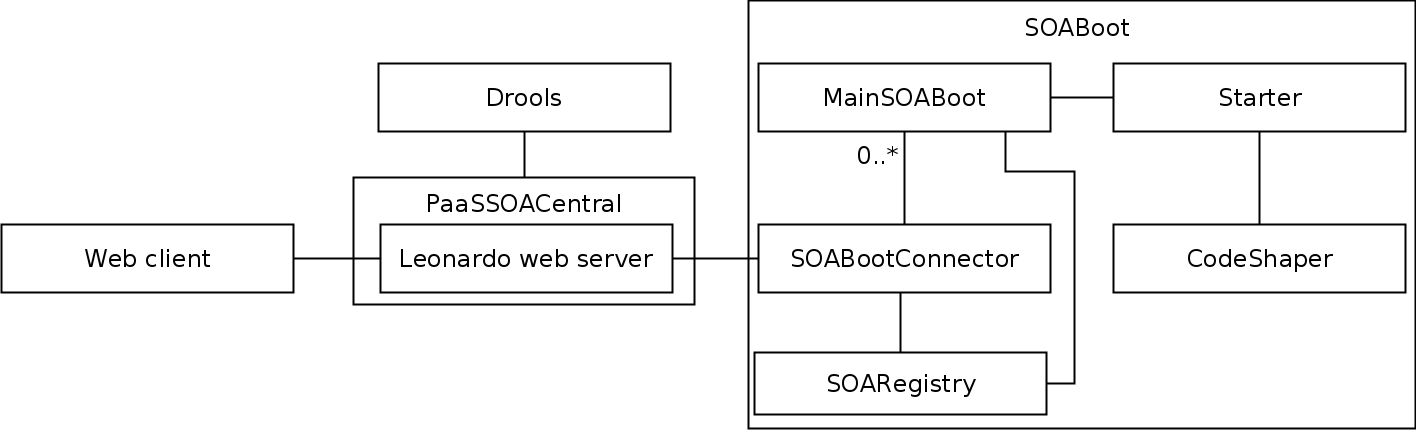
\includegraphics[width=0.8\textwidth]{../figures/jsoa_class_diagram.png}
  \caption{JSOA architecture}
  \label{fig:jsoaArchitecture}
\end{figure}

As seen in \texttt{Figure \ref{fig:jsoaArchitecture}} the architecture of JSOA can be roughly divided into three services (excluding the web client). These services are: Drools, PaaSSOACentral and SOABoot. This section will explain briefly what each service does, and how they communicate with each other. \\

\textbf{Drools} \\
When JSOA starts, the first module to load is Drools. \\
Drools has two main features. The first is to load some libraries which JSOA requires in order to run. The second is event logging. Every time an event happens somewhere in JSOA, it is sent to Drools. Drools also contains a database which meta information about all running services, such as name of deployed input and response time treshold. \\

\textbf{PaaSSOACentral} \\
PaaSSOACentral is the central module of JSOA. After Drools has loaded, PaaSSOACentral is the next thing to start. \\
When the main PaaSSOACentral is started, it starts up the Leonardo\cite{leonardo_website} web server. In addition to the web server, PaaSSOACentral also starts up the SOARegistry, which is used for registering meta information of services (e.g., input and output ports), and the SOABoot connector. The SOABoot connector is used for connecting the Leonardo web server to the main SOABoot. \\
Leonardo acts as a front end to the SOABoot service. When a service is uploaded to JSOA and the "addService" request is received, the web server validates the request, and forwards it to the SOABoot connector. The SOABoot connector fetches meta information for the service from the SOARegistry, and forwards the request to the SOABoot. \\

\textbf{SOABoot} \\
SOABoot is the core service in regards to handling deployed services. When a service is uploaded, started, stopped or deleted, SOABoot is in charge of carrying it out.\\
As seen in \texttt{Figure \ref{fig:jsoaArchitecture}}, SOABoot is divided into five main sub services. MainSOABoot is the main SOABoot service, SOABootConnector is connecting the PaaSSOACentral with the SOABoot and SOARegistry is registering various meta information regarding services. Starter is the service starter service, when a service is stared on JSOA, the Starter is in charge of executing the start commands. The CodeShaper is a sub service of the Starter. When JSOA starts a service, various Jolie service files are generated which JSOA uses to monitor and interact with the service. These files include a surface file, and a wrapper file.\\
In addition to these sub service, SOABoot also connects to a database where every service that is uploaded to JSOA is registered. This data base contains name and status of the service, email address of the service administrator and file name and extension of the uploaded service file.\\

\textbf{Heterogeneity} \\
Notice that in \texttt{Figure \ref{fig:jsoaArchitecture}} that PaaSSOACentral coordinates zero or more SOABoots. This is what makes JSOA excel at extending the framework to a large distributed system, since the developer can easily scale the framework by adding additional SOABoots.\\
As stated above, PaaSSOACentral is the main module of JSOA. When a SOABoot is started, it is attached to the PaaSSOACentral, and when a service is uploaded to JSOA, it is attached to a specific SOABoot.\\
\texttt{Figure \ref{fig:jsoaMultipleSOABoots}} shows a visual representation of how PaaSSOACentral, SOABoot and services are connected.

\begin{figure}[h!]
  \centering
    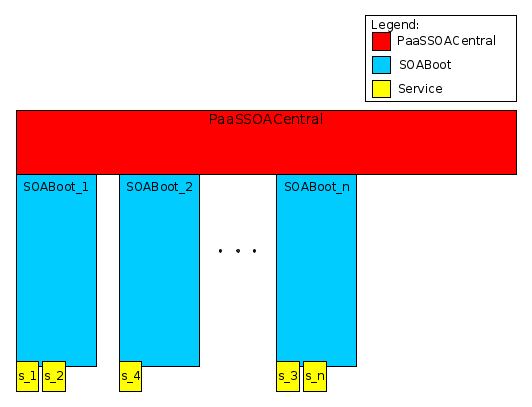
\includegraphics[width=0.8\textwidth]{../figures/jsoa_multiple_soaboot.png}
  \caption{JSOA with multiple SOABoots}
  \label{fig:jsoaMultipleSOABoots}
\end{figure}

When a new SOABoot instance is created, it is connected to a single PaaSSOACentral. When a service is uploaded to JSOA, it is connected to one SOABoot. A single SOABoot can manage many services.\\
Each SOABoot can be thought of as a domain. So if \texttt{Figure \ref{fig:jsoaMultipleSOABoots}} was a website, with multiple web services running, each SOABoot can be considered a domain or sub domain of the web site, or one SOABoot could even be a whole different web site that is hosted on the same server.

\newpage
\begin{figure}[h!]
  \centering
    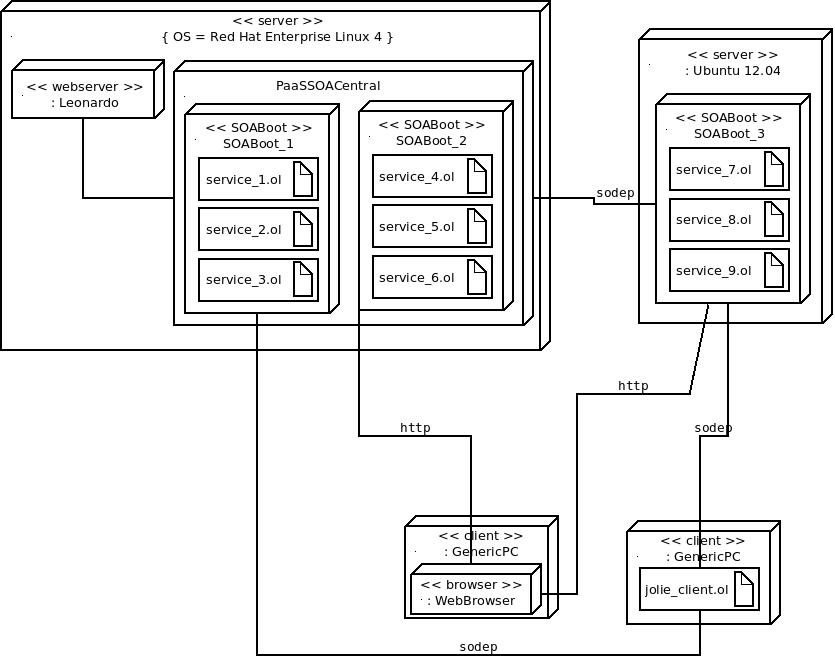
\includegraphics[width=0.8\textwidth]{../figures/jsoa_deployment_diagram.jpeg}
  \caption{JSOA deployment diagram}
  \label{fig:jsoaDeploymentDiagram}
\end{figure}

\texttt{Figure \ref{fig:jsoaDeploymentDiagram}} shows a possible deployment diagram for JSOA.\\
As shown in the diagram, the Red Hat Linux server runs PaaSSOACentral and has two SOABoots running with three services running on each SOABoot. The Ubuntu server has one SOABoot running, with three services running. The SOABoot on the Ubuntu server is connected to the PaaSSOACentral of the Red Hat server.\\
The two clients interact with the services on both servers, via their respective SOABoots.\\

This diagram shows how scalable JSOA is. Imagine that the SOABoots on the Red Hat server allows developers to deploy services written in Python, while the Ubuntu server allows the running of Jolie and Java services. One could add another SOABoot, either on one of the existing servers or a new server, which allows the running of software written in PHP and Ruby. Each of these SOABoots could share the same authentication procedure or alternatively they could all have their own.\\
The diagram gives a good picture on how well JSOA handles scalability, with the ability to build large distributed frameworks, while still coordinating it all from a central location. \\

\newpage
\textbf{Adding a service} \\
There are two ways a user can upload a service to JSOA. The first way is to upload a single Jolie (\textless servicaName\textgreater .ol) file. The second way is to use a \texttt{jap} file.\\
A jap file essentially is a jar file which is recognized by JSOA. The jap file can contain a single Jolie service file, or it can contain a more complex service with multiple folders and files. If there is more than one file, or the main Jolie service does not have the same name as the jap file, JSOA requires that a manifest file is present.

\begin{lstlisting}[caption={Jap file manifest},label={lst:japManifest}]
Manifest-Version: 1.0                                                                                                                                                                                        
X-JOLIE-Main-Program: main.ol                                                                                                                                                                                
X-JOLIE-Options: Options here 
\end{lstlisting}

\texttt{Listing \ref{lst:japManifest}} shows how a jap manifest is structured.\\
The first line is just auto generated information. Line two tells JSOA where the main Jolie service file is found (e.g., main.ol). Line three is for additional options, e.g., command line arguments for the main Jolie service.\\
When a jap file is uploaded to JSOA, it first looks for the manifest file in order to find the main jolie service, this service is then registered in JSOA. If there is no manifest, JSOA tries to find the main service with the same name as the jap file.

\begin{figure}[h!]
  \centering
    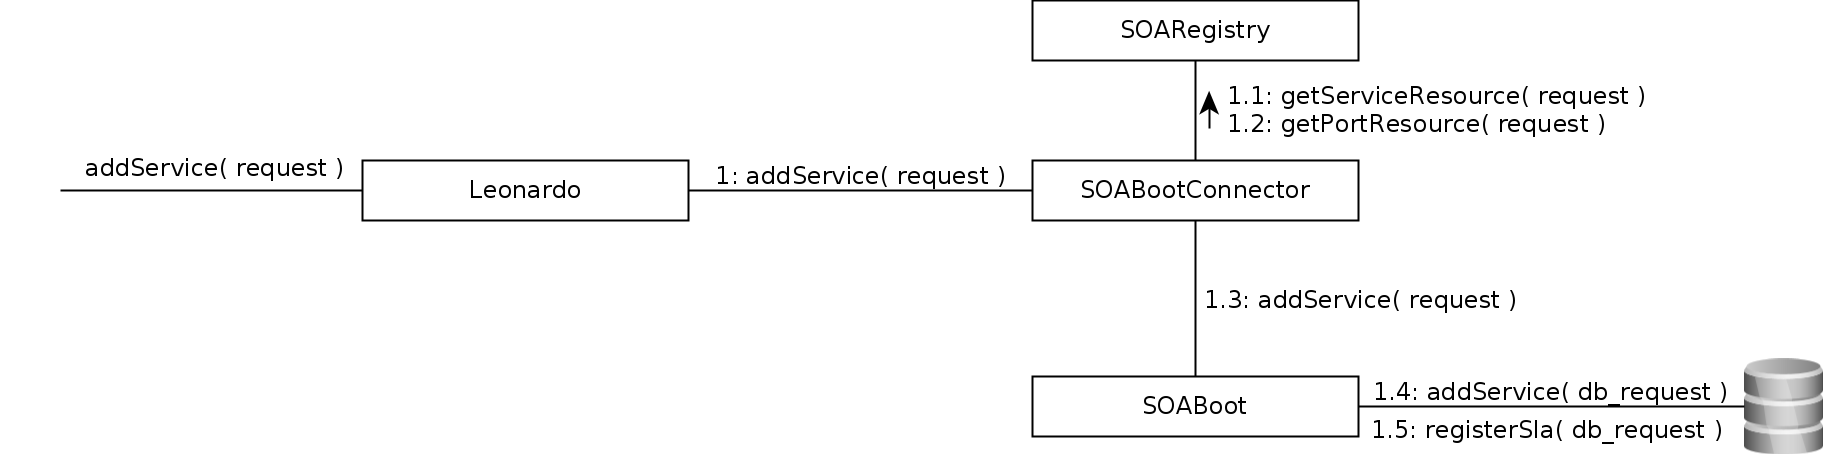
\includegraphics[width=1.0\textwidth]{../figures/jsoa_add_service_communication_diagram.png}
  \caption{Add service}
  \label{fig:jsoaAddService}
\end{figure}

\texttt{Figure \ref{fig:jsoaAddService}} shows a communication diagram, describing what happens when a user uploads a service to JSOA. \\
The first step is that the web client sends the uploaded file, along with the name of the service and the email address of the administrator, to the Leonardo web server. The web server checks the uploaded file to see if it is valid. Checks are made to make sure that the file type is valid and has the correct extension. After the file has been confirmed to be valid, Leonardo parses the file to see if the syntax is correct and all required attributes (e.g., input port and main function) of the service are in place. If any of these tests fail, a FaultException is sent back to the client. \\
Assuming that all tests have passed, Leonardo creates a request, based on the uploaded service, and sends it to the SOABootConnector. \\

The SOABoot connector readies the service for deployment. Service related resources are fetched from the SOARegistry (e.g location and domain of the SOABoot). The SOABoot parses the input file in order
to the get input/output ports of the uploaded service, and sets the location (domain) according to the location/domain of the SOABoot. \\
With this information in place, a new request is created and sent to the main SOABoot. \\

The main SOABoot is where the service is actually added to JSOA. \\
The first thing that happens is that the SOABoot checks if the service exists. Since JSOA requires that services have unique names, SOABoot checks the service database to see if a service already exists with the same name as the newly uploaded service. Assuming that it does not exist, SOABoot creates a working directory for containing the uploaded file, and writes the uploaded file to the directory. After this, a few more checks are made to make sure the service file is valid and does not contain any error. \\
Assuming the file is error free, the next step is to register the service in the database. The service is added to the service database of the SOABoot. Some additional information is also inserted into the SLA database of the Drools. \\
Finally, a console directory is created for the service. This directory is used for logging interactions with the new service. \\

\newpage
\textbf{Starting / deploying a service}
\begin{figure}[h!]
  \centering
    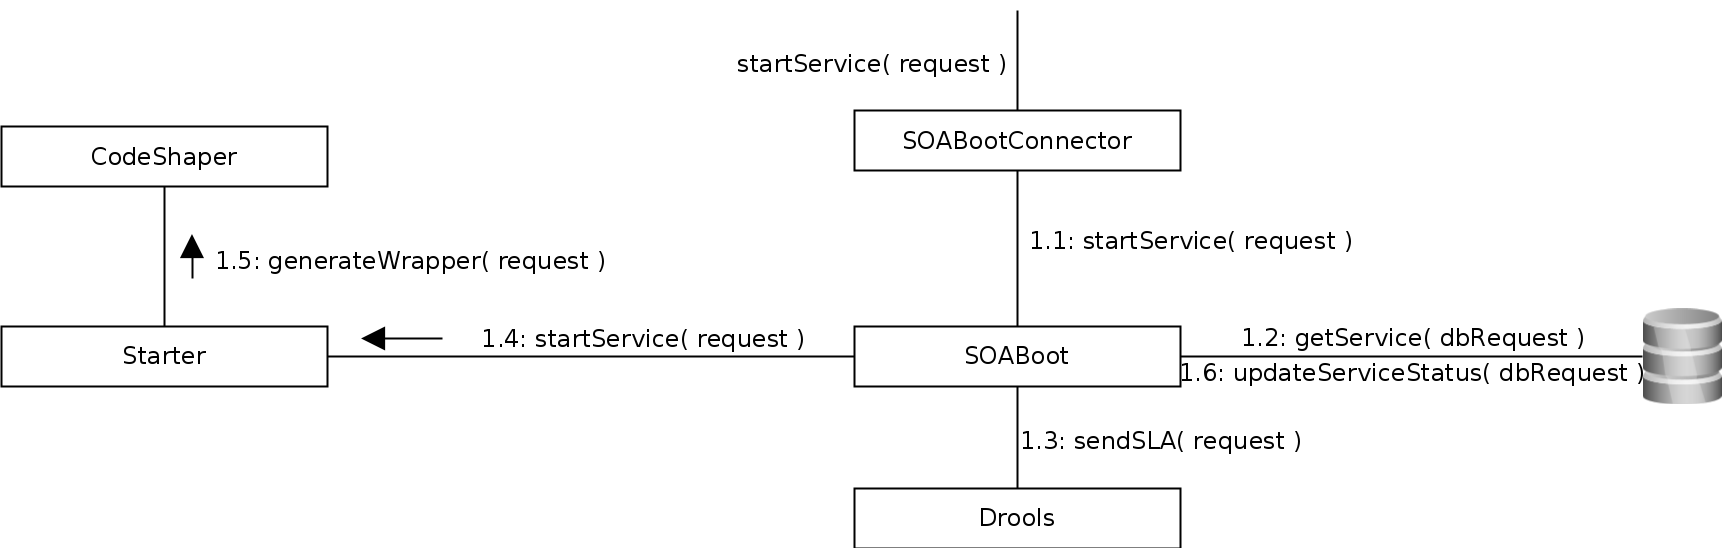
\includegraphics[width=1.0\textwidth]{../figures/jsoa_start_service_communication_diagram.png}
  \caption{Start service}
  \label{fig:jsoaStartService}
\end{figure}

As \texttt{Figure \ref{fig:jsoaStartService}} shows, the communication flow of the start service action is very similar to when adding a new service (\texttt{Figure \ref{fig:jsoaAddService}}). \\
The web client sends start command to the SOABoot connector. The SOABoot connector, like with the add service, fetches information about the service from SOARegistry (e.g., ports), and sends the request to the main SOABoot. \\

SOABoot again makes various tests to see if the service is valid.  \\
Information about the service is fetched from the database, and the service file is parsed by the SOABoot. The parsing of the file includes setting the location of the input ports, based on the SOABoot domain. Updated information about the service is sent to Drools. \\
After this, the request is sent to the main starter which handles the actual work on deploying the service. \\

The startService on the main starter first creates a deployer directory for the service. This directory contains all files related to the deployed service as long as the service is running (the directory is deleted after the service is stopped, and recreated when the service is restarted). The main starter then starts to "unwrap" the service. Here there are two options. The first is if the service is a Jolie file (e.g., \textless serviceName\textgreater .ol file) or the service is a jap file. \\
If the service is a jap file, the first thing that the starter does is copy the jap file into the newly created deployer directory where the jap is extracted. The next step is to find the main Jolie file. This has been specified in the manifest file, so the starter parses the manifest file in order to find the main Jolie file, along with some extra (optional) parameters (e.g., command line arguments for the main Jolie file).  \\
After these steps, the rest is handled like a regular Jolie file. \\

At this stage, JSOA writes a new file based on the uploaded service. This file is the upload service, with the addition of a few input ports and operations which allow JSOA to interact with the service. These operations include a monitor which allows JSOA to get statistics and consoles from the running service. \\
After writing the "monitor-file" JSOA generates a "surface" file. This file is basically a modification of the uploaded service. The changes are made to make it easier for JSOA to fetch input ports and interfaces by altering the names and merging all interfaces to a single interfaces. This surface file is what is exposed to the clients. \\

After the surface, JSOA generates a wrapper file for the service. The wrapper file contains input- and output ports which allows JSOA to interact with the running service. In addition, the wrapper file contains some additional functions, the "shutDown" is an example. The wrapper file is in a way the central file of the service. JSOA communicates with the wrapper file in order to interact with the service and the monitor file. The wrapper file is also the entry point for when clients are using the service. The main input port of the wrapper file embeds the uploaded service, thus allowing clients to interact with the service via the wrapper file.\\

Having generated these files, the service is registered in the SOARegistry.\\
JSOA then fetches the input ports to be deployed and sets the location of the input port based on the current SOABoot domain.\\

The actual deployment phase relies on executing shell\cite{shell_website} commands. \\
The first command is to generate joliedoc\footnote{Example of joliedoc for the "console.iol" service:\\ http://www.jolie-lang.org/?top\_menu=documentation\&sideMenuAction=jsl/Console} for the service. Joliedoc generates an html files which contains the API for that particular service. \\
JSOA then creates a shell script which is in charge of starting the service as well as creating log file for the service. \\
Finally, the shell file is executed, and the service is running.\\

After the service has started, the starter returns back to the main SOABoot. The SOABoot updates the database with information that the service is now running. An entry is also added to the Drools database, informing it about the deployed input port. \\

\textbf{Stopping a service} \\
Stopping a running service on JSOA is more or less the opposite of starting a service.
The web client sends a stop request to the SOABootConnector, which validates the request and passes it on to the main SOABoot. \\
The main SOABoot fetches the service meta data from the SOARegistry (e.g., ports). JSOA then sets the location of the Admin input port of the wrapper file (the one which is in charge of shutting down the service) and executes the shutDown command. \\

After shutting down the service, the service (along with its ports) are removed from the SOARegistry. \\
When the service is remove from the registry, the deployment files and directory are removed.
The stop event is sent to Drools to inform that the service has been stopped, and the SOABoot database is updated with information about the new state of the service.

\subsubsection{JSOA on Windows}\label{subsec:JSOAOnWindows}
As stated in the problem description, the first contribution to the project is to port JSOA to the Windows platform. Since JSOA is based on Java, the foundation was already in place for porting it to Windows.\\
Before JSOA can run on Windows, some changes need to be made. Most of the changes are not related to JSOA, but with the underlying Jolie code. The first change is regarding Windows file paths.  \\

\textbf{Issue \#1: Windows file paths} \\
JSOA is written for the Linux platform, and on Linux the standard file path uses forward slashes \verb|(/some/path/)| but on Windows the default path uses backward slashes \verb|(C:\some\path\).| When the Jolie interpreter is parsing a file path, an exception is thrown because of an illegal index in the file path (e.g., the backslash). \\

The issue appears when JSOA tries to access some files, and the Java code will not accept the backslashes.

\begin{lstlisting}[caption={Windows file path issue},label={lst:windowsFilepathIssue}]
// Linux ( original )
String filename = new File(argsList.get( i )).getCanonicalPath();
// Windows work around 1
String filename = new File(argsList( i )).toURI().toString();
// Windows work around 2
filename = filename.replace( "\\", "/" );
\end{lstlisting}

As seen in \texttt{Listing \ref{lst:windowsFilepathIssue}}, there are two ways to solve this issue. The first solution is to get the URI of the file, and use the URI as the file path (line 4). The second solution is simply to replace the backslashes with forward slashes (line 6). \\
The second solution is used for two reasons. The first is that it is very simple, and does not need to alter the existing code but just add a single line of code after the original. The second is that this solution also works if given only a file path (e.g., a String object, not a File object). If the first solution was used then first required to create a file based on the file name, and then implement the solution. \\
One of the drawbacks of this solution is that the original file path might contain backslashes (as an escape character for white spaces for example). This should not happen, because Java deals with the white spaces, but only extensive testing, which lies outside of the scope of this thesis, can verify if this will happen or not. \\

\newpage
\textbf{Issue \#2: Jap relative file paths} \\
The second issue is related to relative file paths and jap files. \\
Jolie services, like most other programming languages, use so called "include" statement to import code from other files in to the current file. An example of an include statement which includes a file from its parent folder is presented in \texttt{Listing \ref{lst:jolieIncludeStatement}}
\begin{lstlisting}[caption={Jolie include statement},label={lst:jolieIncludeStatement}]
include "../someFile.iol"
\end{lstlisting}
In a regular Jolie service, this does not pose any problems, even on Windows. The problem is when using JSOA jap files. \\

\begin{wrapfigure}{l}{0.35\textwidth}
  \begin{center}
    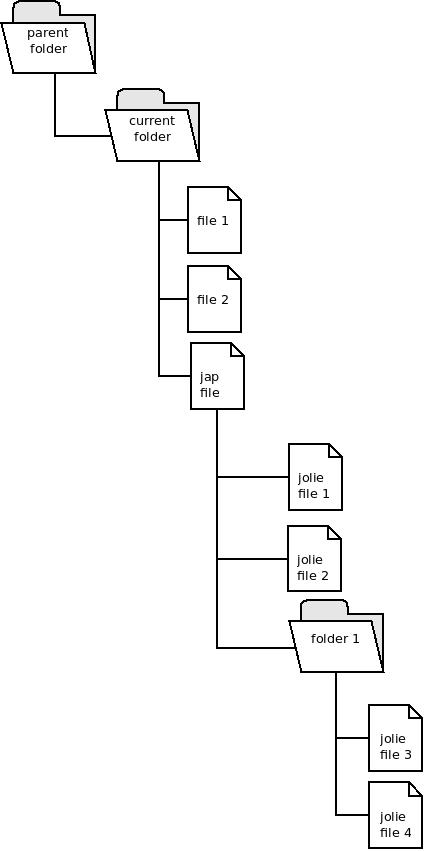
\includegraphics[width=0.3\textwidth]{../figures/jolie_jap_include_issue_graph.jpeg}
  \end{center}
  \caption{Jap file include issue}
  \label{fig:japIncludeIssue}
\end{wrapfigure}

\texttt{Figure \ref{fig:japIncludeIssue}} shows the structure of a file system. Current folder is the folder that we are currently working in. Jap file is the jap file that is uploaded to JSOA. Inside the jap file are two Jolie files, jolie\_file1 and jolie\_file2 and an additional folder folder 1. Inside folder 1 are two additional Jolie files, jolie\_file3 and jolie\_file4. \\
 ~\\ ~\\ ~\\ ~\\ ~\\ ~\\ ~\\ ~\\ ~\\ ~\\ ~\\ ~\\ ~\\ ~\\ ~\\
The jolie\_file3 starts with some include statements:
\begin{lstlisting}[caption={Include statements},label={lst:jolieTwoIncludeStatements}]
1 include "jolie_file4"
2 include "../jolie_file1"
\end{lstlisting}

The first line executes as it should, since the included file is in the same directory as the source file. However, the second line poses an issue. \\
Ordinarily, the statement "../" "means go back one folder". In Windows, a jap file is not considered to be a folder and therefore produces unexpected results. Instead of going from Folder 1 and back to Jap file to look for the file to include, it assumes that we are in the "Current folder" and therefore goes back to the "parent folder" to look for the file to include. Since the target file doesn't exist in the Parent folder, a null pointer exception is raised. \\
In order to get the correct file to include, the parser first needs to get the absolute path of the source file (jolie\_file3). When the absolute path is found, the parser will then create new absolute paths to the include files. \\

The code snippet in \texttt{Listing \ref{lst:japIncludeIssue}} creates absolute file paths based on the relative file paths in the include statements. \\
The path (line 2) is the absolute path to the Jolie file \\
(e.g., \verb| C:\some\path\jolieService.ol| ), while the filename (line 3) is the filename to include (e.g., \verb| ../someOtherJolieFile.ol|).\\
Lines 4-5 convert the path to work with JSOA (replace backslashes with forward slashes). Lines 6 - 11 are creating the actual absolute path. As long as the filename starts with "../", it is removed from the filename, at the same time the last folder is removed from the path. Finally the filename is appended to the path, creating the absolute path to the include path.\\
Lines 20 - 34 do the same thing, only when the include file starts with "./" (e.g., this folder).

\begin{lstlisting}[caption={Fix for jap file include paths},label={lst:japIncludeIssue}]
if(filename.startsWith( "../") ) {
	String tmpPath = path;
	String tmpFilename = filename;
	if(!tmpPath.contains( "/" ) && tmpPath.contains( "\\" )) 
		tmpPath = tmpPath.replace( "\\", "/" );
	while(tmpFilename.startsWith( "../" )) {
		tmpFilename = tmpFilename.substring( 2 );
		if(tmpPath.endsWith( "/" )) 
			tmpPath = tmpPath.substring(0, tmpPath.length() -1);
		tmpPath = tmpPath.substring(0, tmpPath.lastIndexOf( "/" ));
	}
	String tmpUrl = new StringBuilder()
		.append( tmpPath )
		.append( tmpFilename ).toString();
	try {
		url = new URL(
			tmpUrl.substring( 0,4 ) + 
			tmpUrl.substring( 4 ));
	} catch(Exception exn) { }
	} else if(filename.startsWith( "./" )) {
		String tmpPath = path;
		String tmpFilename = filename;
		if(!tmpPath.contains( "/" ) && tmpPath.contains( "\\" )) 
			tmpPath = tmpPath.replace("\\", "/");
		tmpFilename = tmpFilename.substring(1);
		if(tmpPath.endsWith( "/" )) 
			tmpPath = tmpPath.substring(0, tmpPath.length() -1);
		String tmpUrl = new StringBuilder()
			.append( tmpPath )
			.append( tmpFilename ).toString();
		url = new URL(
			tmpUrl.substring( 0,4 ) + 
			tmpUrl.substring( 4 ));
}
\end{lstlisting}

\textbf{Issue \#3: Jolie built-in includes} \\
This issue arises when a service is deployed, and JSOA parses the uploaded file for the input ports of the service. As stated earlier, JSOA generates a wrapper file for the uploaded service. When generating this file, JSOA takes advantage of some libraries that are built-in to Jolie.\\
When parsing "regular" include statements (such as the one in \texttt{Listing \ref{lst:JolieRegularIncludeStatement}}) the, MetaJolie\footnote{MetaJolie is part of the Jolie installation. The MetaJolie class is in charge of the meta information of services, one of which is the include statements} class first checks the current directory to see if the file is found. If not, then it checks the built-in Jolie library. The issue here is that the default Jolie installation directory on Linux (e.g., /opt/jolie/include/) is hard coded into the MetaJolie parser.

\begin{lstlisting}[caption={Jolie regular include statement},label={lst:JolieRegularIncludeStatement}]
include "console.iol"
\end{lstlisting}

Since this is a fundamental bug with Jolie, and therefore outside the scope of this project, a temporary fix is put in place by adding the default Windows installation directory to the MetaJolie parser. This will of course cause the same problem if Jolie is installed in any directory other than the default, but this will be fixed in a later version of Jolie so the problem will be resolved.\\

\textbf{Issue \#4: Shell commands} \\
The final thing which needs adapting to the Windows platform is the execution of services and various commands. \\
As stated in \texttt{section \ref{subsec:JSOA}} the Starter executes shell commands when starting services. These commands need to be fitted for the Windows command prompt.
When starting a service, JSOA creates a bash\footnote{Born again shell. Referring to the Linux default shell.} script which is in charge of starting the services, as well as creating directories and log files. In addition to starting services, JSOA uses the shell for extracting the content of jap files and generating API documentation for the service.\\
\texttt{Listing \ref{lst:linuxWindowsStartCommand}} shows the differences between creating and executing start commands in Linux and Windows.\\
Lines 1 - 11 show how the shell (Linux) commands are created and executed, while lines 13 - 23 show the same thing on the command prompt (Windows).

\begin{lstlisting}[caption={Linux \& Windows starter commands},label={lst:linuxWindowsStartCommand}]
// create shell command                                                                                                                                                                                  
with( shell_file ) {                                                                                                                                                                                     
	.filename = current_dir + "/run.sh";                                                                                                                                                               
	.content = "#! /bin/sh\nnow=\"$(date +\"%y%m%d%H%M%S\")\"\nlogfile=../../consoles/" + service_name + "/$now\"_log.txt\"\njolie " + session + "_wrapper.ol > $logfile 2>&1" };                                                                                                                                                                                                       
writeFile@File( shell_file )();                                                                                                                                                                          
                                                                                                                                                                                                             
// execute shell command                                                                                                                                                                                 
cmd = "sh";                                                                                                                                                                                              
cmd.args = "run.sh";                                                                                                                                                                                     
cmd.workingDirectory = current_dir;                                                                                                                                                                      
exec@Exec( cmd )( result ) 

// create Windows command
with( shell_file ) {                                                                                                                                                                                     
	.filename = current_dir + "/run.bat";
	.content = "set now=%date%\nset logfile=..\\..\\consoles\\" + service_name + "\\%now%_log.txt\njolie " + session + "_wrapper.ol > %logfile% 2>&1" };                                                                                                                                                                                                       
writeFile@File( shell_file )();

// execute windows command
cmd = "cmd";                                                                                                                                                                                             
cmd.args = "/c start run.bat";                                                                                                                                                                           
cmd.workingDirectory = current_dir;                                                                                                                                                                      
exec@Exec( cmd )( result )
\end{lstlisting}

In addition to adapting the shell commands to run on Windows, new commands needed to be added in order to start the C\# service. \\
When the starter is extracting the jap file, additional code needed to be added in order to find the C\# service file.

\begin{lstlisting}[caption={Find .exe file in jap},label={lst:findWinService}]
undef( rq );                                                                                                                                                                                   
rq.filename = current_dir + "META-INF/MANIFEST.MF";                                                                                                                                            
readFile@File( rq )( manif );                                                                                                                                                                  
undef( split_req );                                                                                                                                                                            
split_req = string( manifest );                                                                                                                                                                
contains_req = split_req;                                                                                                                                                                      
contains_req.substring = "X-JOLIE-CSHARP-PROGRAM:";                                                                                                                                            
contains@StringUtils( contains_req )( contains_resp );                                                                                                                                         
if( contains_resp ) {                                                                                                                                                                          
	split_req.regex = "X-JOLIE-CSHARP-PROGRAM:";                                                                                                                                               
	split@StringUtils( split_req )( split_res );                                                                                                                                               
	split_req = split_res.result[ 1 ];                                                                                                                                                         
	split_req.regex = "\n";                                                                                                                                                                    
	split@StringUtils( split_req )( split_res );                                                                                                                                               
	trim@StringUtils( split_res.result[ 0 ] )( cSharpFile );                                                                                                                                   
	winServiceFilename = current_dir + cSharpFile }
\end{lstlisting}              

\texttt{Listing \ref{lst:findWinService}} shows the additional code needed to find the .exe file. Lines 1 - 8 reads the file and split it by the "X-JOLIE-CSHARP-PROGRAM:" string, which has been specified in the manifest. If it finds anything, lines 9 - 16 split the string further to find the filename of the .exe file.\\
If the C\# service is found, it needs to be started when the Jolie proxy is started.

\begin{lstlisting}[caption={Start C\# service},label={lst:startWinService}]
// Create and start the c# application                                                                                                                                                                   
    exists@File( winServiceFilename )( winServiceExists );                                                                                                                                               
    if( winServiceExists ) {                                                                                                                                                                                 
        undef( cmd );                                                                                                                                                                                        
        cmd = "cmd";                                                                                                                                                                                         
        cmd.args = "/c start " + winServiceFilename;
        cmd.workingDirectory = current_dir;                                                                                                                                                                  
        exec@Exec( cmd )( result ) };
\end{lstlisting}

\texttt{Listing \ref{lst:startWinService}} shows how the C\# service is started. Notice that it is almost identical to starting a Jolie service.\\

\textbf{Issue \#5: Empty lines in services} \\
One final note regarding JSOA on Windows.\\
When a Jolie service is uploaded to JSOA. it is required that the service file does not contain any empty lines. The reason for this is that when Jolie is parsing the service file, it considers empty lines as end of file, and stops reading. \\
There seems to be an issue with how Windows and Java file readers work together (since this problem does not exist on Linux). To counter this issue, it requires that service developers to not have any empty lines in their Jolie services, at least until the Jolie/Java parser is fixed. 

\subsubsection{C\# Integration}\label{subsec:CSharpIntegration}
The second part of the first contribution to the project is to add the ability to run services written in C\# to run on JSOA and integrate C\# to communicate with Jolie. \\
In order to integrate Jolie with C\#, there are three things that need to be implemented into C\#: Jolie values, the Sodep protocol and input/output ports. This section will go through the implementation of all three, along with examples on how they are used.\\

\textbf{Values} \\
Jolie types are tree like structures (see section \ref{subsec:Jolie}). The types have a root value (which may be empty) and an arbitrary number of children. The children have a value (again, can be empty) and potentially more children. 
\begin{lstlisting}[caption={Jolie type},label={lst:joliePersonType}]
type Person: void {
	.firstName: string
	.lastName: string
	.address: void {
		.streetName: string
		.streetNumber: int
		.zipCode: int
		.city: string } }
\end{lstlisting}
\texttt{Listing \ref{lst:joliePersonType}} shows an example of a person type in Jolie. \\
The root value (Person) is void and contains three children, firstName (string) lastName (string) and address (void). Address has four children, streetName (string), streetNumber (int), zipCode (int) and city (string). \\
The structure of the Jolie types makes it very easy for creating large, complex types. The underlying Value implementation however, is slightly more complicated.\\

\begin{figure}[h!]
  \centering
    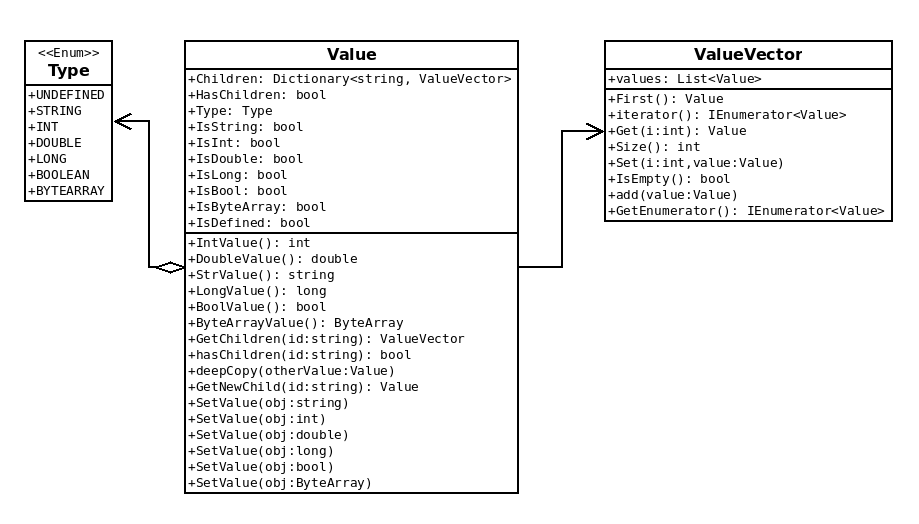
\includegraphics[width=1.0\textwidth]{../figures/cSharpClassDiagram.png}
  \caption{Excerpt from C\# class diagram}
  \label{fig:cSharpClassDiagram}
\end{figure}

\texttt{Figure \ref{fig:cSharpClassDiagram}} shows part of the class diagram for the C\# integration. As the figure shows, Value has a \texttt{type}, this is the type of the data (e.g string, int etc.) The Value also contains a dictionary containing the children of the Value. In the example in \texttt{Listing \ref{lst:joliePersonType}}, this would be firstName, lastName and address. The dictionary does not contain the child value directly but contains a ValueVector which in turn contains a list of values. The reason for the ValueVector containing a list instead of a Value object, is that in Jolie, any data type is a dynamic array (see \texttt{section \ref{subsec:Jolie}}). \\
The rest of the operations on the value objects are used for various checks and to get and set the data of the value. In addition, Value contains a method for copying the Value into another value object (deepCopy\footnote{This is not used in the C\# implementation, but it is used in the Jolie. If the C\# implementation ever will run natively with Jolie (embedded) this will be used}). \\

\begin{lstlisting}[caption={Person type in C\#},label={lst:personTypeInCSharp}]
public class Address {
	public string StreetName { get; set; }
	public int StreetNumber { get; set; }
	public int ZipCode { get; set; }
	public string City { get; set; }
	
	public Address(Value value) { ValueToObj(value); }

	public void ValueToObj(Value value) {
		this.StreetName = value.GetChildren("streetName").First().StrValue;
		this.StreetNumber = value.GetChildren("streetNumber").First().IntValue;
		this.ZipCode = value.GetChildren("zipCode").First().IntValue;
		this.City = value.GetChildren("city").First().StrValue; }
	
	public Value ObjToValue() { /* omitted */ }
}
public class Person {
	public string FirstName { get; set; }
	public string LastName { get; set; }
	public Address { get; set; }
	
	public Person(Value value) { ValueToObj(value); }
	
	public void ValueToObj(Value value) {
		this.FirstName = value.GetChildren("firstName").First().StrValue;
		this.LastName = value.GetChildren("lastName").First().StrValue;
		this.Address = new Address(Value.GetChildren("address").First()); }
	
	public Value ObjToValue() {
		Value retval = new Value();		
		ValueVector fNameVec = new ValueVector();
		fNameVec.add(new Value(FirstName));
		ValueVector lNameVec = new ValueVector();
		lNameVec.add(new Value(LastName));
		ValueVector aVec = new ValueVector();
		aVec.add(Address.ValueToObj());		
		retval.Children.Add("firstName", fNameVec);
		retval.Children.Add("lastName", lNameVec);
		retval.Children.Add("address", aVec;		
		return retval; } }
\end{lstlisting}

\texttt{Listing \ref{lst:personTypeInCSharp}} shows how the person type in \texttt{Listing \ref{lst:joliePersonType}} is implemented in C\#. \\
Each Jolie Value object\footnote{"Jolie Value object" refers to a Jolie Value in C\#} contains two methods. One to convert Jolie values to C\# object, and one to convert C\# objects to Values. In the example above, the Person type is created by first getting the child from the dictionary with the key "firstName" (line 25). Note that they key is the same as the variable name in the Jolie implementation. Since \texttt{value.GetChildren} returns a ValueVector, it then needs to get the first element in the \emph{values} list of the ValueVector, and finally extract the string value.\\
The rest of the object is created the same way. Note however that when creating the \texttt{Address} object, the child Value of the original Value object, containing the "address" Value, is sent to the Address object (line 27) to handle in the same way as explained here. \\

When converting from C\# object to Value, the procedure is the same but the other way around (line 29 - 40).
Create a ValueVector, and add the Value to the values list of that ValueVector. Like before, the Address value is created by delegating the conversion to the Address object which then creates the required structure.\\
When finished with all ValueVectors, they are all added to the Values children.

\begin{lstlisting}[caption={Using C\# Values},label={lst:usingCSharpValues}]
Person p = new Person(value);
p.ValueToObj(value) // is called implicitly in the constructor.
Value v2 = p.ObjToValue();
\end{lstlisting}

\texttt{Listing \ref{lst:usingCSharpValues}} shows how simple it is to convert a Value to a C\# object (line 1 - 2) and vice versa (line 3).\\

When implementing the Value, the ByteArray needed to be implemented as well. The ByteArray basically is just a wrapper class around a regular ByteArray, which contains some helper methods to make it easier to interact with. \\

\textbf{Sodep} \\
In order to make the communication between C\# and Jolie as smooth as possible, the Sodep protocol needed to be implemented in C\#. Since the Sodep protocol uses CommMessages to transfer data, naturally, the CommMessage needed to be implemented first.\\
A CommMessage is basically a wrapper around a message sent via Sodep. CommMessage contains five fields:
\begin{itemize}
\item\textbf{Id}\\
The id of the CommMessage
\item\textbf{OperationName}\\
This is the operation the CommMessage is calling to invoke. In C\#, this could be translated to be a method call at the destination.
\item\textbf{ResourcePath}\\
The resource path is used for redirection in Jolie\cite{jolie_redirection}. Since this feature is not used in JSOA at all, this is not implemented in C\#.
\item\textbf{Value}\\
The value is, as described earlier in this section, the actual data that is sent with the CommMessage.
\item\textbf{FaultException}\\
The FaultException is the default exception used in Jolie. In C\#, it is derived from the Exception\cite{cSharp_exception}. FaultException contains a name (fault name) and a value.
\end{itemize}

\newpage
\begin{figure}[h!]
  \centering
    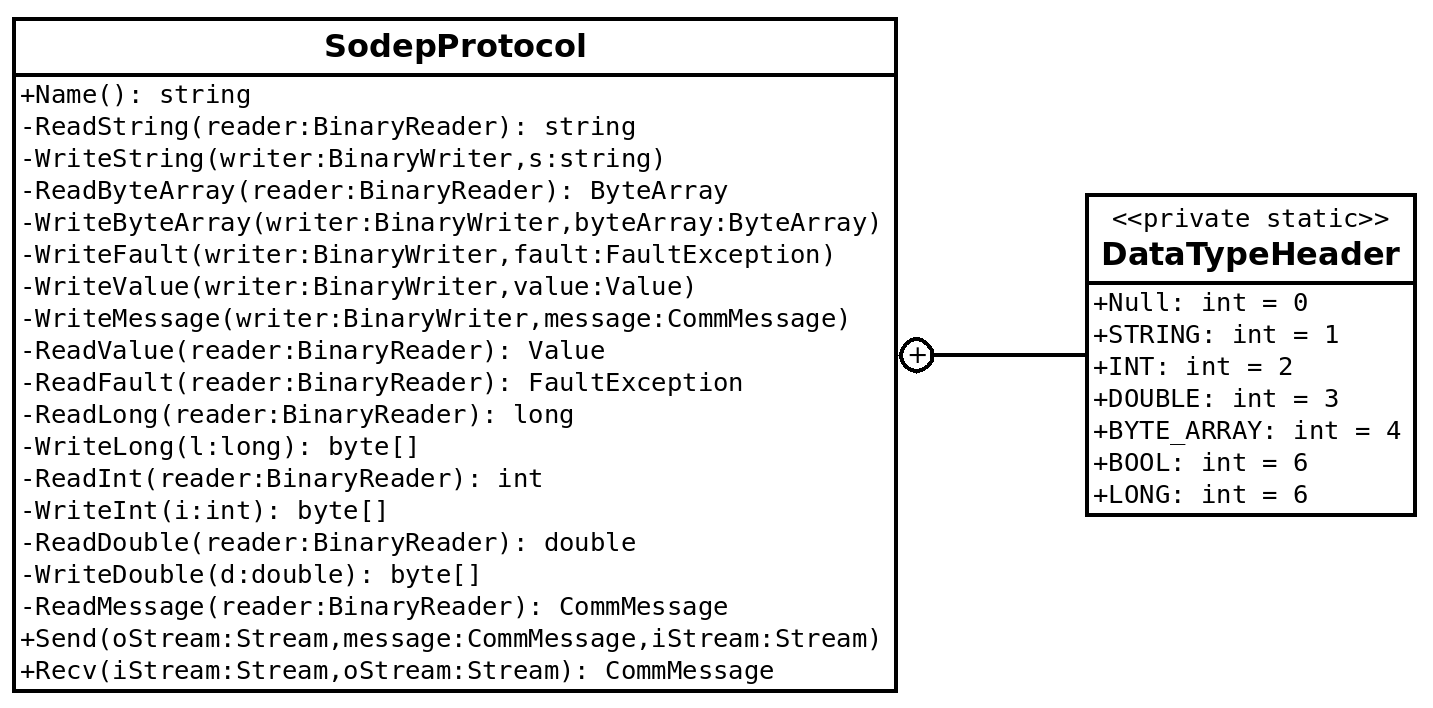
\includegraphics[width=1.0\textwidth]{../figures/sodepClassDiagram.png}
  \caption{Sodep protocol class overview}
  \label{fig:sodepClassDiagrams}
\end{figure}

The Sodep protocol has two public methods, Send and Recv, along with multiple private helper methods (\texttt{Figure \ref{fig:sodepClassDiagrams}}). The public methods are used for sending and receiving CommMessages, while the private methods help to write the various data to the stream.\\
In addition, the SodepProtocol class also contains the private class DataTypeHeader, this is used for determining what data type to read/write next (string, int etc).\\
Writing string values is pretty straight forward. The string is converted to a byte array\footnote{Byte array here is a regular C\# byte array and not the Jolie implementation}. The length of the byte array is then sent to the stream, followed by the byte array itself. The receiving end is pretty similar, first read the length of the byte array, then read the byte array, and finally convert it to its string representation.\\
Dealing with number types (int, double and long) is slightly more complicated. Usually it is pretty simple to read and write number types since the BinaryReader/Writer have read/write methods for all these data types. However, since Sodep (the Jolie implementation) deals in big endian\cite{endian_definition} and C\# deals in little endian, there are some issues. Without going into too much detail about endianness, what it does is that they read/write bytes in opposite order. Because of this, the data would not make any sense on the receiving end, and the reader would crash. To counter this, a couple of helper methods are implemented.

\newpage
\begin{lstlisting}[caption={Little- big endian Int32 converter method},label={lst:endianHelpMethods}]
private int ReadInt(BinaryReader reader) {
	byte[] arr = reader.ReadBytes(4);
	Array.Reverse(arr);
	return BitConverter.ToInt32(arr, 0); }
 
private byte[] WriteInt(int i) {
	byte[] arr = BitConverter.GetBytes(i);
	Array.Reverse(arr);
	return arr; }
\end{lstlisting}

\texttt{Listing \ref{lst:endianHelpMethods}} show how the data is converted. When the data comes in, the bytes are read into a byte array (line 2). The byte array is then reversed (line 3) and then converted to its data type (line 4). When sending data the opposite is done.\\

Most of the SodepProtocol methods are pretty simple. What they do is read and write data to the NetworkStream using Binary readers/writers. The most complex of the read/write methods, are the read/write value methods. \texttt{Listing \ref{lst:writeValueExcerpt}} shows how the WriteValue method is implemented.

\begin{lstlisting}[caption={WriteValue excerpt},label={lst:writeValueExcerpt}]
private void WriteValue(BinaryWriter writer, Value value) {                                                                                                                  
	try {                                                                                                              
	if (value.IsString) {                                                                                                          
		writer.Write((byte)DataTypeHeaderId.STRING);                                                           
		WriteString(writer, value.StrValue);	}
	else if( ... ) // Rest of write data methods ommited
	Dictionary<string, ValueVector> children = value.Children;                                                 
	LinkedList<KeyValuePair<string, ValueVector>> entries = 
		new LinkedList<KeyValuePair<string, ValueVector>>();
	foreach (KeyValuePair<string, ValueVector> entry in children) {                                                                                                          
		entries.AddLast(entry);                                                                                
	}                                                                                                                                                                                                                                     
	writer.Write(WriteInt(entries.Count));                                                                                                                                                                                                
	foreach (KeyValuePair<string, ValueVector> entry in entries) {                                                                                                          
		WriteString(writer, entry.Key);                                                                        
		writer.Write(WriteInt(entry.Value.Size()));                                                            
		foreach (Value v in entry.Value)	{                                                                                                      
			WriteValue(writer, v);                                                                             
		}                                                                                                      
	}                                                                                                          
	} catch (IOException e) { }                                                                                      
}                       
\end{lstlisting}

The WriteValue first sends the data type of the root value to the stream (string in the example), followed by the actual data\footnote{The sending of the other data types have been omitted in order to save space} (line 4 - 5). When the data is sent, all children of the values are fetched and added to a list and the amount of children in sent to the stream (line 7 - 13).\\
Finally the method loops through all the children, sending their key (variable name) followed by the amount of children (line 15 - 16). Each child Value is then sent by recursively calling the WriteValue method (line 17 - 19).\\
The procedure on the receiving end is basically the reverse of the writing (see \texttt{appendix \ref{app:ReadValue}} for the ReadValue implementation). \\

\textbf{Input and output ports} \\
In an attempt to stay true to the Jolie structure, input port and output ports are implemented. Implementation of the ports is not critical for the communication with Jolie, but in order to simplify the services, and to save developers from having to implement communication media (e.g., sockets) for each service, the ports are implemented.\\

\begin{figure}[h!]
  \centering
    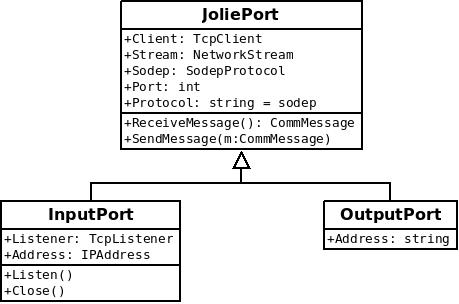
\includegraphics[width=0.8\textwidth]{../figures/PortClassDiagram.jpeg}
  \caption{Input and output port class diagram}
  \label{fig:portClassDiagram}
\end{figure}

As \texttt{Figure \ref{fig:portClassDiagram}} shows, the ports are very simple.\\
The base port, \texttt{JoliePort}, contains all the properties and methods which are common for both ports. \texttt{Client} is used for sending data, via its \texttt{Stream}. \texttt{SendMessage} and \texttt{ReceiveMessage} are used for sending and receiving CommMessages via the \texttt{SodepProtocol}. The \texttt{Port} specifies which port number the JoliePort will use. \texttt{Protocol} is only used for returning the name of the protocol used, this is pretty redundant in its current state, but if the ports will be extended to support multiple protocols, this will become relevant.\\
InputPort contains two additional properties and methods. \texttt{Listen()} and \texttt{Close()} are used for starting and stopping the inputPort. The \texttt{Listener} listens for incoming connections on the port number specified. The \texttt{Address} property is used for setting the ip address of the input port. In this implementation, the ip address is always local but this might change in the future. \\
The \texttt{OutputPort} contains a single property, namely address. The address is used to specify the location of the InputPort which the output port communicates with.\\

\begin{lstlisting}[caption={Example usage of input/output port in C\#},label={lst:inputOutputPortExample}]
public JoliePort inputPort = new InputPort(8000);
inputPort.Listen();
CommMessage m = inputPort.Recv();
// ... do something with CommMessage

public JoliePort outputPort = new OutputPort("localhost", 8000);
CommMessage m2 = new CommMessage( ... );
outputPort.send(m2);
\end{lstlisting}

These simple construct make it a lot easier for developer to handle communication with Jolie via the Sodep protocol, as can be seen in \texttt{Listing \ref{lst:inputOutputPortExample}}. Depending on the service, listening for incoming request might a bit more complex than this (see \texttt{section \ref{subsec:RunningExample}} for a more thorough example) but essentially, \texttt{Listing \ref{lst:inputOutputPortExample}} shows all that is required of the service developer to handle communication with Jolie using input and output ports. \\

\textbf{C\# interface / abstract class} \\
In order to make life easier for developers, some interfaces and abstract were created. The interface IJolieValue, was created for the data objects. The interface has two methods, to convert a Value to C\# object, and vice versa.\\
The abstract class JolieServiceBase is created in order to aid developers in developing Jolie services. This  abstract class contains all the methods which a service requires to communicate efficiently with Jolie. At this time, there are only two methods, Start() and ShutDown(). The Start() method is used for "starting" the input port, and handling incoming requests (see \texttt{section \ref{subsec:RunningExample}} for a detailed example). The ShutDown() is, as the name states, used for shutting down the C\# service.\\
As the C\#-Jolie library will grow, and additional functionality is added, this abstract class will grow.

\begin{figure}[h!]
  \centering
    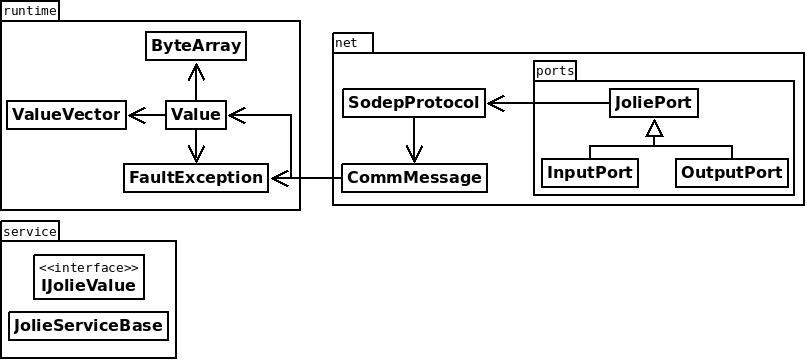
\includegraphics[width=0.8\textwidth]{../figures/fullCSharpClassDiagram.jpeg}
  \caption{Jolie C\# class diagram}
  \label{fig:fullCSharpClassDiagram}
\end{figure}

\texttt{Figure \ref{fig:fullCSharpClassDiagram}} shows a complete class diagram of the C\# implementation of Jolie. Properties and methods are omitted for clarity.


\subsubsection{Authentication}\label{subsec:Authentication}
As stated in the problem description, the second contribution the project is to implement authentication to JSOA. Currently, JSOA does not offer any form of authentication, so any form of authentication is tied to each individual service.\\

When implementing the authentication, the preferable method is that the uploaded service shall not be affected by the authentication in any way. To put it in other words, the authentication must be entirely based on the framework, completely independent of the running service. \\

There were a few options considered on how to implement the authentication. \\
The first option is to implement it in the Sodep protocol. The way this would be done is to add authentication data (e.g username and password or some authentication token) to the CommMessages sent via the Sodep protocol. This data could then be handled by the main inputport of JSOA before being forwarded to the relevant service. \\
The main upside of this solution is that the developer would not have to worry  about the authentication, since it all happens on a lower level. One of the drawbacks of using this method is that it limits JSOA to only use the Sodep protocol. Since JSOA (Jolie) supports multiple communication protocols\cite{jolie_protocols}, this would severely limit JSOA. To counter this, authentication data could be added to every protocol which JSOA supports, but doing so is a lot of work, which in turn is hard to maintain. Another drawback is that it makes the protocol a lot more complex which can cause problems and maybe performance issues as well. \\

The other method discussed (the one used) is to use courier sessions\footnote{See \texttt{section \ref{subsec:Jolie}} for more details on courier sessions}. Courier sessions allow the extension of existing types and handling of those extensions independently of the services' handling of the original request. For example if a request from a client is sent to a service running on JSOA only contains an int, using a courier session, authentication data can be added to the request and handled before handling the actual request. After handling the authentication, the field is removed from the request (going back to the original request) and the request forwarded to the intended service. \\
\texttt{Listing \ref{lst:simpleJolieData}} and \texttt{\ref{lst:jolieDataWithAuth}} show how the request looks like with and without authentication data on the client side.
\begin{lstlisting}[caption={Simple Jolie data},label={lst:simpleJolieData}]
type Request: void { .x: int }
\end{lstlisting}

\begin{lstlisting}[caption={Simple Jolie data with authentication key},label={lst:jolieDataWithAuth}]
type Request_auth: void { .x: int .key: string }
\end{lstlisting}

\texttt{Listing \ref{lst:jolieCourier}} in \texttt{Section \ref{subsec:Jolie}}, shows how the courier session looks like on the service side. The example in \texttt{Listing \ref{lst:jolieCourier}} shows that the input port aggregates an output port with an \texttt{Interface extender}. This allows the input port to add the authentication data to the incoming request. The courier session then handles the authentication data, removes it, and forwards the request to the output port.

\begin{figure}[h!]
  \centering
    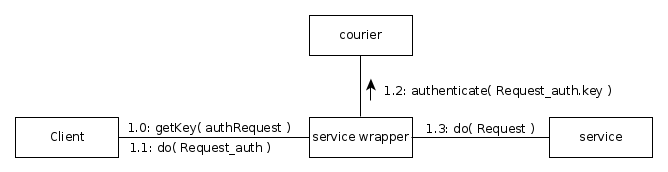
\includegraphics[width=0.8\textwidth]{../figures/jsoa_generic_authentication_communication_diagram.png}
  \caption{JSOA communication diagram with authentication}
  \label{fig:jsoaAuthArchitecture}
\end{figure}

\begin{figure}[h!]
  \centering
    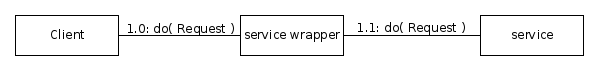
\includegraphics[width=0.8\textwidth]{../figures/jsoa_generic_no_authentication_communication_diagram.png}
  \caption{JSOA communication diagram without authentication}
  \label{fig:jsoaNoAuthArchitecture}
\end{figure}

~\\
As seen in \texttt{Figure \ref{fig:jsoaAuthArchitecture}} and \texttt{Figure \ref{fig:jsoaNoAuthArchitecture}} the authentication has added one layer of indirection.\footnote{Note that the courier is actually attached to the services wrapper but has been shown separately in the diagram for clarity.} In \texttt{Figure \ref{fig:jsoaNoAuthArchitecture}}, a request is sent from the client to the service wrapper, and is then forwarded to the service, which then does the work and returns through the same path. \\
\texttt{Figure \ref{fig:jsoaAuthArchitecture}} contains additional operations. First the client sends a "getKey" request to the service wrapper. The service wrapper validates the request to see if the user has access or not (usually username and password). If valid, the service wrapper returns an authentication key to the client. The client then sends a "do" request to the service wrapper. Unlike \texttt{Figure \ref{fig:jsoaNoAuthArchitecture}} here the client sends an extended request (Request\_auth in the example) instead of a regular request. The extended request is the same as the regular, but with added authentication data (see \texttt{Listing \ref{lst:simpleJolieData} and \ref{lst:jolieDataWithAuth}}). When the extended request is received by the wrapper, the courier session starts. The courier session checks if the key is valid. If the key is valid, the courier session removes the authentication data from the extended request (making it a regular request) and forwards the regular request to the service. If the key is invalid, the courier returns a fault exception and the operation terminates. \\

Only a few lines of code are required to implement this solution. Since the service wrapper (which is the main entry point for the running service) is generated at runtime, the courier session, along with the authentication data and the interface extender, is added to the code shaper, which generates the wrapper file.

\begin{lstlisting}[caption={Adding courier to service wrapper},label={lst:courierToWrapper}]
[ prepareWrapper( request )( response ) {                                                                                                                                                              
/* ... */
wrapper = wrapper + "type AuthenticationData: void {\n";                                                                                                                                         
wrapper = wrapper + ".key: string \n";                                                                                                                                                           
wrapper = wrapper + "}\n";                                                                                                                                                                                                                                                                                                                                                                                    
wrapper = wrapper + "interface extender AuthInterfaceExtender {\n";                                                                                                                              
wrapper = wrapper + "RequestResponse: *( AuthenticationData )( void ) \n";                                                                                                                       
wrapper = wrapper + "OneWay: *( AuthenticationData ) \n";                                                                                                                                        
wrapper = wrapper + "}\n"; */                                                                                                                                                                    
/* ... */
wrapper = wrapper + "interface __WrapperInterface {\n";                                                                                                                                          
/* ... */
// Add authentication to the wrapper interface                                                                                               
wrapper = wrapper + "getKey( string )( string )\n"; 
/* ... */
wrapper = wrapper + "inputPort Admin {\n";                                                                                                                                                       
/* ... */
wrapper = wrapper + "Interfaces: __WrapperInterface\n";                                                                                                                                          
wrapper = wrapper + "Aggregates: Monitor, " + request.input[ deployed_input[ 0 ] ].name.name + " with AuthInterfaceExtender";

wrapper = wrapper + "courier Admin {\n";                                                                                                                                                         
wrapper = wrapper + "[ interface " + request.input[ deployed_input[ 0 ] ].name.name + "Interface( request )( response ) ] {\n";                                                                  
wrapper = wrapper + "if( request.key == \"auth_valid\" ) {\n";                                                                                                                                   
wrapper = wrapper + "forward " + request.input[ deployed_input[ 0 ] ].name.name + "( request )( response )\n";                                                                                   
wrapper = wrapper + "}\n}\n}\n";

wrapper = wrapper + "main {\n";                                                                                                                                                                  
/* ... */
wrapper = wrapper + "[ getKey( username )( key ) {\n";                                                                                                                                           
wrapper = wrapper + "if( username == \"username\" ) {\n";
wrapper = wrapper + "key = \"auth_valid\"\n";                                                                                                                                                    
wrapper = wrapper + "} else {\n";                                                                                                                                                                
wrapper = wrapper + "key = \"auth_invalid\"\n";                                                                                                                                                  
wrapper = wrapper + "}\n";                                                                                                                                                                       
wrapper = wrapper + "} ]{ nullProcess }\n";
\end{lstlisting}

\texttt{Listing \ref{lst:courierToWrapper}} shows how the authentication is implemented. Lines 3 - 9 define the AuthenticationData and the InterfaceExtender. The interface extender extends all requests with the authentication data. Line 14 adds the "getKey" method to the \_\_WrapperInterface. On line 19, the Admin input port (which is the main input port to the uploaded service) aggregates the deployed service input port (which has been converted to an output port by JSOA) with the interface extender. What this does is to extend every incoming request with the interface extender.\\
Lines 21 - 25 defines the actual courier session. Note that on line 22 \emph{request.input[
deployed\_input[ 0 ] ].name.name} is the name of the interface for the service. The courier checks if the key, which is the extended authentication data, matches a certain valid key ("auth\_valid" in the example). If it does match, the request is forwarded to the aggregated output port (line 24).\\
Lines 29 - 35 add the "getKey" method to the main function, which allows the client to authenticate and get the valid key. Since the example is just a proof-of-concept, "getKey" just checks if the username matches the string "username". In reality, this is where the actual authentication takes place (check if username and password match some database entry for example).\\

Using this method has a lot of advantages.  \\
The complexity of the authentication algorithm can easily be extended or changed. All that needs changing is the courier session and the "getKey" operation on the service side.(\texttt{Listing \ref{lst:courierToWrapper}}:29-35).\\
Another upside with this method is that it is completely tied to the SOABoot. If a developers wishes to extend the JSOA framework further, using a different authentication method, all that is needed to be done is to edit the SOABoot, and connect another instance of the SOABoot to the PaaSSOACentral.\\
As mentioned before, the major upside of using this method, is that it is completely independent of the deployed service. This allows the developer of a service to implement it any way he wants without being concerned about authentication. The only part which needs to be aware of the authentication, is the client connecting to the service. \\

As with most software solutions, there are drawbacks. One of the drawbacks is that every service uploaded to this instance of SOABoot is required to use the same authentication procedure. Even if a service is deployed which is not intended to have any authentication, it will have to handle it. This can be countered by coding the key into the client. Doing this makes it seem like there is no authentication (from the users perspective) even if there is.\\
Even if every service is tied to this authentication, there is no stopping the developers of the services to add additional authentication to the service.

\subsection{Running example}\label{subsec:RunningExample}
The third and final contribution is to develop a proof-of-concept service, written in C\#, which will be used to evaluate the changes made to JSOA.\\
The service will consist of a C\# service, a Jolie proxy which will handle the communication between JSOA and the C\# service, and a client\footnote{See \texttt{appendix \ref{app:exampleClient}}} written in Jolie.

\begin{lstlisting}[caption={TwiceRequest and TwiceResponse in Jolie},label={lst:twiceDataJolie}]
type TwiceRequest: void { .x: int }
type TwiceResponse: void { .y: int }
\end{lstlisting}

The example service is divided into two parts. The first part deals with simple data. It takes a TwiceRequest and returns a TwiceResponse. \texttt{Listing \ref{lst:twiceDataJolie}} shows the Jolie implementation of the TwiceRequest and TwiceResponse. The service will take the number from the request, double it, and return it to the Jolie client.\\

The second part of the service demonstrates how the C\# service can handle complex data by simulating a database application. The service takes a Person request (\texttt{Listing \ref{lst:joliePersonType}} shows the Jolie implementation of the Person type) and allows the client to get, insert or delete persons from a database.\footnote{The service does not use an actual database but a list of Person objects to simulate database behaviour.}

When the C\# service starts, it first initializes the input port by specifying the port number to listen on (\texttt{Listing \ref{lst:initWinService}}). The actual service is then started, in this example it is started on a new thread.

\begin{lstlisting}[caption={Initialize C\# service},label={lst:initWinService}]
public class Program {                                                                                                                                                                                                        
	public static int port;                                                                                                                                                                              
	public static void run() {                                                                                                                                                                                                    
		Twice t = new Twice(port);                                                                                                                                                                       
		t.Start(); }                                                                                                                                                                                                    
                                                                                                                                                                                                             
	public static void Main(string[] args) {
		port = 9998;                                                                                                                                                                             
		Thread th = new Thread(new ThreadStart(run));                                                                                                                                            
		th.Start(); } }
\end{lstlisting}

After the input port has been initialized, it starts to listen for incoming connections.\\
When a request is received, the service enters a switch. The cases of the switch is the operation name of the incoming CommMessage. Each operation name corresponds to a method in the C\# service (\texttt{Listing \ref{lst:winServiceSwitch}}).

\begin{lstlisting}[caption={C\# service start method},label={lst:winServiceSwitch}]
public override void Start() {                                                                                                                                                                                                    
  while (true) {                                                                                                                                                                                                
    if (InputPort.Listener.Pending()) {                                                                                                                                                                                            
      InputPort.Listen();                                                                                                                                                                      
      try {                                                                                                                                                                                        
        CommMessage m = InputPort.ReceiveMessage();                                                                                                                                          
        if (m != null && m.Value != null) {                                                                                                                                                                                    
          switch (m.OperationName.ToLower()) {                                                                                                                                                                                
            case "twice":                                                                                                                                                                
              handleTwice(m);                                                                                                                                                          
              break;                                                                                                                                                                   
            case "insert":                                                                                                                                                               
              handleInsert(m);                                                                                                                                                         
              break;                                                                                                                                                                   
            case "get":                                                                                                                                                                      
              handleGet(m);                                                                                                                                                                
              break;                                                                                                                                                                       
            case "delete":                                                                                                                                                                   
              handleDelete(m);                                                                                                                                                             
              break;                                                                                                                                                                       
            case "shutdown":                                                                                                                                                             
              handleShutDown();                                                                                                                                                        
              break; } }                                                                                                                                                                                    
            InputPort.Close(); }                                                                                                                                                                                        
            catch (Exception) {  } } } }
\end{lstlisting}

\texttt{Listing \ref{lst:handleGet}} shows what happens when the "get" request is received in the input port.\\
First the Jolie value is converted to a C\# object, \texttt{Listing \ref{lst:personTypeInCSharp}} shows how the conversion between Jolie value and C\# objects is implemented.\\
When the value is converted, the service does what ever work it is designed to do. In this example, it gets a Person from a database. \\
When the operation is done, the object is converted into a Jolie Value, and returned back to the client, in a CommMessage, via the Sodep protocol.

\begin{lstlisting}[caption={Handle get method},label={lst:handleGet}]
private void handleGet(CommMessage m) {                                                                                                                                                                                                    
	PersonDB db = new PersonDB();                                                                                                                                                                    
	Person person = new Person(m.Value);                                                                                                                                                             
	PersonResponse resp = new PersonResponse(db.Get(person));                                                                                                                                        
	InputPort.SendMessage(new CommMessage(m.Id, m.OperationName, m.ResourcePath, resp.ObjToValue(), m.IsFault ? m.Fault : null)); }
\end{lstlisting}

As can be seen from this example, the communication with Jolie is very simple to implement once the Jolie-C\# library is in place. The only thing the developer needs to worry about to implement (regarding the Jolie communication) is the switch in the start method (\texttt{Listing \ref{lst:winServiceSwitch}}).\\
Note that even though there is no sign of any authentication, this service uses the authentication discussed in \texttt{section \ref{subsec:Authentication}}. 

\begin{figure}[h!]
  \centering
    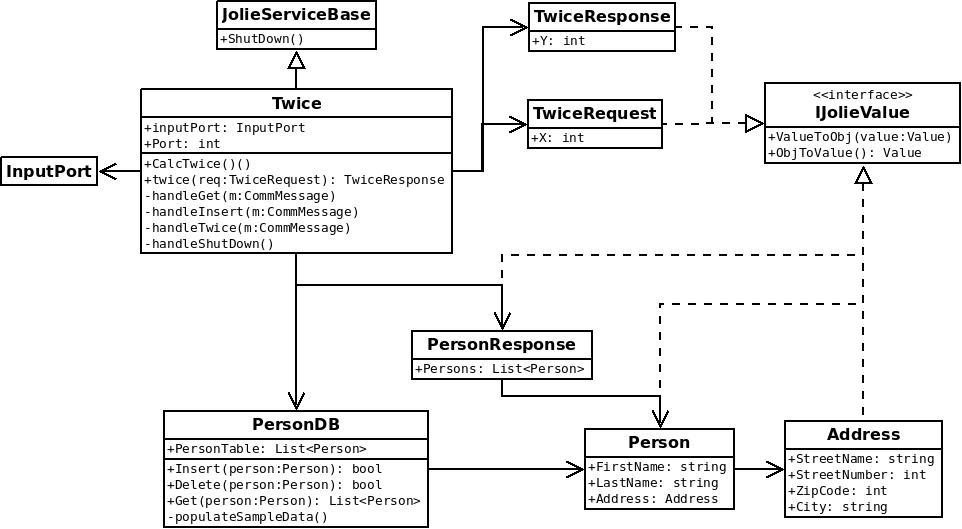
\includegraphics[width=0.8\textwidth]{../figures/exampleServiceClassDiagram.jpeg}
  \caption{Example service class diagram}
  \label{fig:exampleServiceClassDiagram}
\end{figure}

\texttt{Figure \ref{fig:exampleServiceClassDiagram}} shows a complete class diagram of the example service.

Before the C\# service is ready to upload to JSOA, a Jolie proxy needs be implemented. This proxy handles the communication between JSOA and the C\# service.

\begin{lstlisting}[caption={Jolie-C\# proxy},label={lst:JolieCSharpProxy}]
type Person: void { ... }                                                                                                                                                                                                            
type PersonResponse: void { ... }
type TwiceRequest: void { ... }                                                                                                                                                                                                            
type TwiceResponse: void { ... }                                                                                                                                                                                                            
interface twiceInterface { ... }                                                                                                                                                                                                            
interface personInterface { ... }                                                                                                                                                                                                            
outputPort proxy {                                                                                                                                                                                           
           Location: "socket://localhost:9998"                                                                                                                                                               
           Protocol: sodep                                                                                                                                                                                   
           Interfaces: twiceInterface, personInterface }                                                                                                                                                                                                            
inputPort twiceIP {                                                                                                                                                                                          
          Location: "local"                                                                                                                                                                                  
          Protocol: sodep                                                                                                                                                                                    
          Aggregates: proxy }                                                                                                                                                                                                            
main { linkIn( nothing ) }   
\end{lstlisting}

\texttt{Listing \ref{lst:JolieCSharpProxy}} shows the proxy for the C\# service example\footnote{"linkIn( nothing )" inside the main function just means that it does nothing, but just forwards the request}. Note that the implementation of the types and interfaces have been omitted in order to save space, but the implementation is matching the types and methods in the C\# service.\\
How this works is that the output port proxy, is the output port which communicates with the C\# service (note that the Location is the same as the one in the C\# service). The input port is how JSOA communicates with the service. The Location of the input port is set by JSOA.\\
With the proxy in place, the service is ready to be uploaded to JSOA. 

When uploading the service, all related files need to be put inside a jap file. 

\begin{lstlisting}[caption={Updated jap file manifest},label={lst:updatedManifest}]
Manifest-Version: 1.0                                                                                                                                                                                        
X-JOLIE-Main-Program: proxy.ol                                                                                                                                                                                
X-JOLIE-CSHARP-PROGRAM: TwiceService.exe                                                                                                                                                                     
Comment_X-JOLIE-Options: Options here     
\end{lstlisting}

\texttt{Listing \ref{lst:updatedManifest}} shows the manifest required for the jap file in this example. Compared to the manifest file in \texttt{Listing \ref{lst:japManifest}}, there is one extra line. This line \emph{(X-JOLIE-CSHARP-PROGRAM: TwiceService.exe)} tells JSOA where to find the main C\# service file. Note that the main Jolie file in this manifest file is the proxy service.

\begin{figure}[h!]
  \centering
    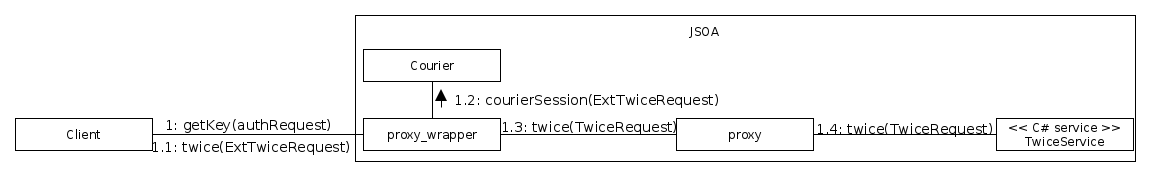
\includegraphics[width=0.8\textwidth]{../figures/example_service_communication_diagram.png}
  \caption{Example service communication diagram}
  \label{fig:exampleServiceCommunicationDiagram}
\end{figure}

\texttt{Figure \ref{fig:exampleServiceCommunicationDiagram}} shows a communication diagram of the example service deployed on JSOA. Notice that compared to \texttt{figure \ref{fig:jsoaAuthArchitecture}}, there is an extra layer of indirection, namely the proxy. 


\subsection{Benchmarking}\label{subsec:Benchmarking}
The second part of the third contribution is to evaluate the JSOA framework in order to evaluate potential performance changes after the extra layers of indirection have been added because of the C\# service and the authentication (see \texttt{figure \ref{fig:jsoaAuthArchitecture}} and \texttt{\ref{fig:exampleServiceCommunicationDiagram}}). \\
The full tables with all the results can be found in the SVN repository mentioned in the preface.\\

\textbf{Benchmarking methodology}\\
In order to do the evaluations, some benchmarking needs to be done. This is done by uploading two versions of the same service, one written in Jolie and one written in C\# with a Jolie proxy.

\begin{lstlisting}[caption={Jolie implementation of the TwiceService},label={lst:jolieTwice}]
type TwiceRequest:void { .x: int }
type TwiceResponse: void { .y: int }
interface twiceInterface { 
	RequestResponse: twice( TwiceRequest )( TwiceResponse ) }
inputPort mainIP { /* ... */ }
main { twice( req )( resp ) { resp.y = req.x * 2 } }
\end{lstlisting}

\texttt{Listing \ref{lst:jolieTwice}} shows the Jolie implementation of the service used for the benchmarking. The service takes a TwiceRequest, doubles the number (x) and returns a TwiceResponse.\\

The actual benchmarking is divided into two parts, first both the Jolie and C\# services test how much time difference there is when sending requests which are authenticated every time, compared to just authenticating the first request\footnote{Authentication in this context refers to the "getKey" request. The courier session is evaluated on every request regardless}. This test simulates a client sending a single request, and then closes. The second part simulates a client that connects to the service, fetches the authentication key and stores it for all additional requests.\\

The second test is to measure the time difference between the calling the Jolie service compared to the C\# service. Since the C\# service has one extra layer of indirection compared to the Jolie service (\texttt{figure \ref{fig:jsoaAuthArchitecture}} and \texttt{\ref{fig:exampleServiceCommunicationDiagram}}), the intuition is that the C\# service should take a little longer.

\begin{lstlisting}[caption={Benchmark client},label={lst:benchmarkClient}]
main {                                                                                                                                                                                                       
	/* .. prepare file for result export */
	request.x = 55;                                                                                                                                                                                         
	for( i = 0, i < 100, i++ ) {                                                                                                                                                                            
		getCurrentTimeMillis@Time()( startTime );                                                                                                                                                          
		getKey@twiceOP( "username" )( request.key );                                                                                                                                                       
		twice@twiceOP( request )( response );                                                                                                                                                              
		getCurrentTimeMillis@Time()( endTime );                                                                                                                                                            
		time = endTime - startTime;                                                                                                                                                                        
		timeArray[i] = time;                                                                                                                                                                               
		undef( startTime ); undef( endTime ); undef( time ); 
		undef( response )                                                                                                                                                                                  
	};                                                                                                                                                                                                    
	/* .. write file with results */                                                                                                                                                                                                      
}
\end{lstlisting}

\texttt{Listing \ref{lst:benchmarkClient}} shows the client used for the benchmarking. Note that the types, interface and output port have been omitted for clarity (see \texttt{appendix \ref{app:exampleClient}} for the full implementation).\\
The client sends 100 requests to the service and times how long it takes to make each request. These results are then written to a file to be processed later. \\
Notice that on line 6, the "getKey" call is inside the loop. In the second part of the test (where the request is evaluated only once), the "getKey" is outside the loop.\\

When all tests are finished, both for the Jolie and C\# services, the results are processed. The processor finds the time difference between the Jolie and the C\# service, as well as the request with authentication and the one without. In addition to finding the difference, the average time it takes to make a request is calculated.\\

\begin{lstlisting}[caption={Result processor excerpt},label={lst:benchmarkProcessor}]
public static void main( String[] args ) { ... }
public static String compare( int[] arg1, int[] arg2, int[] arg3 )
{ ... }
public static double getAverage( int[] arr ) { ... }
public static void writeFile(String filename, String content)
{ ... }
\end{lstlisting}

\texttt{Listing \ref{lst:benchmarkProcessor}} shows an excerpt of the result processor. It takes two parameters, the result files from two of the tests mentioned above, along with an optional third parameter which is the name output file for the processed results.\\
The Compare method takes three arrays. The first two arrays are the results from the input files which are inserted into an array in the main method. The third array is the combined result. The getAverage method calculates the average time it takes to send a request to the service. The final method, writeFile, is optional. If an output file has been specified, this method writes the results to the output file.\\

\textbf{Benchmarking results}\\
This section will analyse the results of the benchmarking.\\
It should be noted that the actual time it takes to handle a request might not be 100\% accurate. The reason for this is that there are multiple factor which can affect the performance. For one thing, the server runs locally so any time it takes to send the request via the network (internet) is not taken into account. The second thing is that there are multiple other processes running on the same computer which might use some resources, causing the results to be incorrect. However, what is interesting in these tests is the difference between the two cases studied. Since both cases are run on the same computer, under the same circumstances, these test should give a fair picture of what the difference in performance looks like.\\

\newpage
\textbf{Authentication vs no authentication}\\
The first benchmark measures how long it takes to handle a request when the request is authenticated every time, compared to when the request is authenticated once, and then the same authentication key is used in the following requests.

\begin{table}[h!]
\begin{center}
\begin{tabular}{ | c | c | c | }
\hline
No auth (ms) & Auth (ms) & Compared (no auth - auth) (ms) \\ \hline
  9  &  37  &  -28  \\ \hline                                                                                                                                                                                
  4  &   3  &    1  \\ \hline                                                                                                                                                                                
  4  &   4  &    0  \\ \hline                                                                                                                                                                                
  9  &   4  &    5  \\ \hline                                                                                                                                                                                
  5  &   3  &    2  \\ \hline                                                                                                                                                                                
  4  &   3  &    1  \\ \hline                                                                                                                                                                                
  4  &   3  &    1  \\ \hline                                                                                                                                                                                
  6  &   6  &    0  \\ \hline                                                                                                                                                                                
  ... & ... & ... \\ \hline
  avg. 3.7 & avg. 3.69 & avg. 0.01 \\ \hline 
\end{tabular}
\label{table:jolieAuthResults}
\caption{Excerpt of benchmark results of Jolie service authentication vs no authentication}
\end{center}
\end{table}

\texttt{Table 1} shows an excerpt of the results of the first test for the Jolie service. As seen in the third column (combined) there is very little difference between the two. Sometimes the request with authentication is slightly faster and sometimes the other is faster.\\
As it also can be seen by the average, the request with authentication is 0.01 ms faster, which in practice means that they are identical.\\
Notice that the first request of the second column it takes 28ms longer than the one in the first column. This is because Jolie closes the connection after some time has passed and it takes a bit longer to open the connection again. This can be seen throughout the full table.

\newpage
\begin{table}[h!]
\begin{center}
\begin{tabular}{ | c | c | c | }
\hline
No auth (ms) & Auth (ms) & Compared (no auth - auth) (ms) \\ \hline
 30  &  39  &  -9  \\ \hline                                                                                                                                                                                 
  5  &   5  &   0  \\ \hline                                                                                                                                                                                 
 10  &   4  &   6  \\ \hline                                                                                                                                                                                 
  9  &   5  &   4  \\ \hline                                                                                                                                                                                 
  7  &   5  &   2  \\ \hline                                                                                                                                                                                 
  5  &   8  &  -3  \\ \hline                                                                                                                                                                                 
  4  &   5  &  -1  \\ \hline                                                                                                                                                                                 
  7  &   7  &   0  \\ \hline
  ... & ... & ... \\ \hline
  avg. 3.49 & avg. 3.8 & avg. -0.31 \\ \hline 
\end{tabular}
\label{table:winAuthResults}
\caption{Excerpt of benchmark results of C\# service authentication vs no authentication}
\end{center}
\end{table}

\texttt{Table 2} shows an excerpt of the results of the first test for the C\# service. Much like with the Jolie service, there is very little difference. The first column (no authentication) is slightly faster on average (0.31 ms). This is such a small number that in practice, there is no real difference.\\

Based on these two tests, it can be concluded that even if the authentication has added an extra layer of indirection. and requires the client to make one additional request for the authentication, there is no loss in performance.\\
In practice, when the service is hosted on a remote server, there might be a difference since the extra request takes some time to send to the server via the network (internet).\\

\newpage
\textbf{Jolie service vs C\# service}\\
The second benchmark measures the time difference when using Jolie service compared to C\# services. This test requires that each request is authenticated.
\begin{table}[h!]
\begin{center}
\begin{tabular}{ | c | c | c | }
\hline
Jolie service (ms) & C\# service (ms) & Compared (jolie - C\#) (ms) \\ \hline
 40  &  38  &   2  \\ \hline                                                                                                                                                                                 
  3  &   5  &  -2  \\ \hline                                                                                                                                                                                 
  4  &   3  &   1  \\ \hline                                                                                                                                                                                 
  4  &   4  &   0  \\ \hline                                                                                                                                                                                 
  4  &   5  &  -1  \\ \hline                                                                                                                                                                                 
  4  &   2  &   2  \\ \hline                                                                                                                                                                                 
  3  &   5  &  -2  \\ \hline                                                                                                                                                                                 
  6  &   6  &   0  \\ \hline
  ... & ... & ... \\ \hline
  avg. 3.81 & avg. 3.33 & avg. 0.48 \\ \hline 
\end{tabular}
\label{table:jolieVsWindows}
\caption{Excerpt of benchmark results of Jolie service vs C\# service }
\end{center}
\end{table}

\texttt{Table 3} shows an excerpt of the results of the final test, the comparison between Jolie services and C\# services.\\
This test is a little trickier. On average, the C\# service is a little faster (0.48 ms) but looking at each request separately, the Jolie service is faster in most of the requests. \\
The reason for C\# being faster on average, is that the C\# service keeps the connection open, while the Jolie service closes the connection after some time, and it needs to be opened again before handling the request. \\
Based on this test, it can be concluded that when not taking in consideration the time it takes to open the connection, the Jolie service is faster, but sending multiple requests, which require the connection to reopened from time to time, the C\# service is faster, even if it has an extra layer of indirection.

\newpage
\section{Conclusion}\label{sec:Conclusion}
This thesis set out to create a PaaS cloud framework which is platform independent, allows the deployment of services written in multiple programming languages, especially the larger, commercial programming languages. The framework needed to be scalable in the sense that support for additional programming languages could be added in the future. Finally the framework needed to automatically handle some non-functional aspects, such as authentication.\\

The work shown in this thesis has been built on the existing PaaS framework JSOA\cite{jsoa_website}.\\

JSOA has been extended to run natively on the Windows platform, taking it one step further towards becoming completely platform independent.\\
JSOA has also been extended to support services written in the C\# programming language. Multiple Jolie constructs have been implemented in C\#; Values, input and output ports and the Sodep protocol are noteworthy examples. By this implementation, JSOA now offers support for running services written in C\#.\\

Authentication has also been added to the JSOA framework. The actual authentication algorithm is in a prototype state (e.g., only a static check of a username is made), but the foundation is in place for extending it to production state. This authentication allows service developers to develop services without having to consider authentication into the service architecture.\\

Evaluations showed that there is no noteworthy performance loss caused by the added layers of indirection caused by the authentication and the C\# implementation. Although it should be noted that these evaluations took place on a regular laptop, with the framework running locally.\\
Extensive evaluation of JSOA would be a thesis in itself, but based on the comparison between Jolie and C\# services, both with authentication and without, there is no noteworthy difference in performance.

\subsection{Limitations}\label{subsec:Limitations}
Because of time constraints, there are some limitations and minor issues with the JSOA framework.\\
JSOA offers the ability to get the surface definition to a service, which is used for developing clients to interact with the service. In its current state, the surface definition does not show any signs of the required authentication data, which results in an error when trying to connect to the service. It still is possible to add this authentication data to the client, but unless client developers know the structure of the authentication in JSOA, they have no way of knowing that it is required.\\
This is issue is easily fixed and will be fixed in the future.

\subsection{Future work}\label{subsec:FutureWork}
Extending JSOA is a never ending story. There are always new functionalities, and support for additional platforms and programming languages which can be added, while those existing can be improved. The following section names a few additions which are interesting for the future.\\

\textbf{Automatic generation of the C\# interface} \\
As it is implemented now, every C\# service need to handle the communication with JSOA manually. Although the implementation of input ports and output ports have made it really simple, this can still be improved further. Automatic generation of the interface could easily be implemented by adding some annotations to the C\# library which then can be parsed, and generated automatically.\\

\textbf{Automatic generation of the Jolie proxy}\\
Every C\# service running on JSOA requires a Jolie proxy service which acts as an intermediary between the C\# service and JSOA. This proxy does nothing except forwarding requests from JSOA to the C\# service.\\
Adding a parser and a code generator, this proxy service could easily be automatically generated when the service is deployed. However, this requires that the parser has access to the C\# source code, or at least a strictly defined API of the C\# service. \\

\textbf{Port to OSX platform}\\
Porting JSOA to Windows is one step in making the framework runnable on every major platform (JSOA is already running on Linux).\\
The next step would be to port JSOA to the Mac OSX platform.\\
Since OSX is based on Unix, there should not be too much work to do, but as with the Windows implementation, there might still be some work to do.\\

\textbf{Support for additional programming languages}\\
With the addition of C\#, JSOA now supports deployment of services written in Jolie, Java, JavaScript and C\#. Adding additional programming languages to the list of supported languages would be the next step. Using the methods used in this thesis (implement Sodep, Jolie values and input/output ports) support for additional programming languages can be added to the framework.\\

\textbf{Add compilers}\\
In its current state, JSOA accepts compiled C\# services. Extending JSOA to allow developers to uploaded source files, which can be compiled on the cloud framework could be a huge improvement. Having this option, version control systems (e.g., Git, SVN) can be added to JSOA, making life easier for service developers.\\ 

\textbf{Add domain to the authentication, allowing the deployment of multi-instance services}\\
Adding domains to the authentication procedure allows for the deployment of multi-instance service on JSOA. This would allow developers to upload multi-instance software to the framework, and have JSOA handling the routing for each instance.

\newpage
\begin{thebibliography}{9}

\bibitem{azure_website}
Microsoft Azure website. \texttt{http://azure.microsoft.com/en-us/}

\bibitem{ec2_website}
Amazon EC2 website. \texttt{https://aws.amazon.com/ec2/}

\bibitem{google_app_engine_website}
Google developers. Google app engine. \\
\texttt{https://developers.google.com/appengine/?csw=1}

\bibitem{jsoa_website}
JSOA website. \texttt{http://sourceforge.net/projects/jsoa/}

\bibitem{nist}
NIST website. Cloud computing definition. \\ \texttt{http://www.nist.gov/itl/cloud/upload/cloud-def-v15.pdf}

\bibitem{jolie_website}
Jolie website. \texttt{http://www.jolie-lang.org/}

\bibitem{java_socket_listener}
Java api. Socket listener. \texttt{http://download.java.net/jdk7/archive/
b123/docs/api/java/net/ServerSocket.html}

\bibitem{jolie_protocols}
Jolie website. Supported protocols. \texttt{http://www.jolie-lang.org/
?top\_menu=documentation\&sideMenuAction=protocols/introduction}

\bibitem{leonardo_website}
Leonardo website. \texttt{http://sourceforge.net/projects/leonardo/}

\bibitem{shell_website}
Indiana University website. In Unix, what is the shell?\\
\texttt{http://kb.iu.edu/data/agvf.html}

\bibitem{jolie_redirection}
Jolie website. Redirections. \texttt{http://www.jolie-lang.org/?top\_menu
=documentation\&sideMenuAction=architectural\_composition/redirection}

\bibitem{cSharp_exception}
Microsoft MSDN. Exception API. \texttt{http://msdn.microsoft.com/en-us/library/
system.exception.aspx}

\bibitem{endian_definition}
Webopedia. Big- little-endian. \texttt{http://www.webopedia.com/TERM/B/big\_endian.html}

\bibitem{jolie_locations}
Jolie website. Locations. \texttt{http://www.jolie-lang.org/?top\_menu=
documentation\&sideMenuAction=locations/introduction}

\end{thebibliography}

\newpage
\begin{appendices}
\section{Sodep ReadValue}\label{app:ReadValue}
\begin{lstlisting}[caption={Sodep ReadValue method},label={lst:sodepReadValue}]
private Value ReadValue(BinaryReader reader)                                                                                                                                                         
{                                                                                                                                                                                                    
try {                                                                                                                                                                                                
  Value value = new Value();                                                                                                                                                                   
  byte b = reader.ReadByte();                                                                                                                                                                  
  switch (b) {                                                                                                                                                                                            
    case DataTypeHeaderId.STRING:                                                                                                                                                            
      value = new Value(ReadString(reader)); break;                                                                                                                                                                               
    case DataTypeHeaderId.INT:                                                                                                                                                               
      value = new Value(ReadInt(reader)); break;                                                                                                                                                  
    case DataTypeHeaderId.LONG:                                                                                                                                                              
      value = new Value(ReadLong(reader)); break;                                                                                                                                                 
    case DataTypeHeaderId.DOUBLE:                                                                                                                                                            
      value = new Value(ReadDouble(reader)); break;                                                                                                                                               
    case DataTypeHeaderId.BYTE_ARRAY:                                                                                                                                                        
      value = new Value(ReadByteArray(reader)); break;                                                                                                                                            
    case DataTypeHeaderId.BOOL:                                                                                                                                                              
      value = new Value(reader.ReadBoolean());                                                                                                                                             
      break;                                                                                                                                                                               
    case DataTypeHeaderId.NULL:                                                                                                                                                              
      break;
    default:                                                                                                                                                                                 
      break;                                                                                                                                                                               
  }                                                                                                                                                                                            
  Dictionary<string, ValueVector> children = value.Children;                                                                                                                                   
  string s;                                                                                                                                                                                    
  int n, i, size, k;                                                                                                                                                                           
  n = ReadInt(reader);                                                                                                                                                                         
  ValueVector vec;                                                                                                                                                                             
  for (i = 0; i < n; i++) {                                                                                                                                                                                            
    s = ReadString(reader);                                                                                                                                                                  
    vec = new ValueVector();                                                                                                                                                                 
    size = ReadInt(reader);                                                                                                                                                                  
    for (k = 0; k < size; k++) {                                                                                                                                                                                        
      vec.add(ReadValue(reader)); }                                                                                                                                                                                        
    if (!children.ContainsKey(s)) children.Add(s, vec);}                                                                                                                                                                                            
    return value; }                                                                                                                                                                                                
	catch (Exception e) { return null; } }
\end{lstlisting}

\newpage
\section{Example service client}\label{app:exampleClient}
\begin{lstlisting}[caption={Example service client},label={lst:exampleServiceClient}]
include "console.iol"                                                                                                                                                                                        
include "time.iol"                                                                                                                                                                                           
include "file.iol"                                                                                                                                                                                           
type TwiceRequest:void { .x: int .key: string }                                                                                                                                                                                                            
type TwiceResponse: void { .y: int }                                                                                                                                                                                                            
interface twiceInterface {                                                                                                                                                                                   
          RequestResponse: twice( TwiceRequest )( TwiceResponse ), getKey( string )( string )                                                                                                                
          OneWay: shutdown( void ) }                                                                                                                                                                                                            
outputPort twiceOP {                                                                                                                                                                                         
           Location: "socket://localhost:12001"                                                                                                                                                              
           Protocol: sodep Interfaces: twiceInterface }                                                                                                                                                                                                                                                                                                                                                                                                                         
main {                                                                                                                                                                                                       
     tmpFilename = args[0]; filename = "result/" + tmpFilename + ".txt";                                                                                                                                                            
     exists@File( filename )( fileExists );                                                                                                                                                                  
     if( fileExists ) {                                                                                                                                                                                      
         delete@File( filename )( isDeleted )                                                                                                                                                                
     };                                                                                                                                                                                                      
     timeArray = "";                                                                                                                                                                                         
     content = "";                                                                                                                                                                                           
     request.x = 55;                                                                                                                                                                                         
     for( i = 0, i < 100, i++ ) {                                                                                                                                                                            
          getCurrentTimeMillis@Time()( startTime );                                                                                                                                                          
          getKey@twiceOP( "username" )( request.key );                                                                                                                                                       
          twice@twiceOP( request )( response );                                                                                                                                                              
          getCurrentTimeMillis@Time()( endTime );                                                                                                                                                            
          time = endTime - startTime;                                                                                                                                                                        
          timeArray[i] = time;                                                                                                                                                                               
          undef( startTime ); undef( endTime ); undef( time ); 
          undef( response )                                                                                                                                                                                  
     };                                                                                                                                                                                                                                                                                                                                                                                                                                                                                                                                                                                                                                
     for( j = 0, j < #timeArray, j++ ) {                                                                                                                                                                     
          content = content + timeArray[j] + "\n"                                                                                                                                                            
     };                                                                                                                                                                                                                                                                                                                                                                                                                   
     fileRequest.filename = filename;                                                                                                                                                                        
     fileRequest.content = content;                                                                                                                                                                          
     writeFile@File( fileRequest )() 
}
\end{lstlisting}
\end{appendices}

\end{document}